\documentclass[12pt,a4paper]{article}
\usepackage[a4paper, margin=0.8in, headheight=14pt]{geometry}
\usepackage{fontspec}
\usepackage{unicode-math}
\setmainfont{TeX Gyre Pagella}
\setmonofont[Scale=0.88]{TeX Gyre Cursor}
\setmathfont{Latin Modern Math}
\usepackage{xcolor}
\usepackage{colortbl}
\usepackage{titlesec}
\usepackage{enumitem}
\usepackage{tabularx}
\usepackage{booktabs}
\usepackage{array}
\usepackage{amsmath}
\usepackage{tikz}
\usetikzlibrary{shapes.geometric, arrows.meta, positioning, calc, fit, decorations.pathreplacing, decorations.pathmorphing}
\usepackage{tcolorbox}
\tcbuselibrary{skins, breakable}
\usepackage{hyperref}
\usepackage{fancyhdr}
\usepackage{graphicx}
\usepackage{microtype}
\hyphenpenalty=10000
\exhyphenpenalty=10000
\sloppy
\usepackage{caption}
\usepackage{setspace}
\usepackage{multirow}
\usepackage{tocloft}
\newcommand{\Q}[1]{\textbf{#1}\par\noindent\ignorespaces}
\definecolor{myred}{RGB}{196,30,58}
\definecolor{mydark}{RGB}{30,30,50}
\definecolor{mygreen}{RGB}{14,120,80}
\definecolor{myteal}{RGB}{0,130,140}
\definecolor{myamber}{RGB}{180,100,0}
\definecolor{mypurple}{RGB}{100,30,160}
\definecolor{mygray}{RGB}{246,247,249}
\definecolor{mgframe}{RGB}{180,185,200}
\definecolor{watermark}{RGB}{145,150,170}
\definecolor{hdrred}{RGB}{250,232,235}
\definecolor{hdrgreen}{RGB}{220,244,233}
\definecolor{hdrteal}{RGB}{220,242,244}
\definecolor{hdramber}{RGB}{253,242,215}
\definecolor{hdrpurple}{RGB}{238,228,255}
\definecolor{hdrgray}{RGB}{238,240,245}
\definecolor{rowalt}{RGB}{250,251,253}

\titleformat{\section}{\large\bfseries\color{myred}}{\thesection.}{0.5em}{}[\vspace{1pt}{\color{myred}\rule{\linewidth}{0.8pt}}]
\titleformat{\subsection}{\normalsize\bfseries\color{myteal}}{\thesubsection}{0.5em}{}
\titlespacing*{\section}{0pt}{18pt}{7pt}
\titlespacing*{\subsection}{0pt}{11pt}{4pt}
\setlength{\parindent}{0pt}
\setlength{\parskip}{4pt}
\renewcommand{\cfttoctitlefont}{\large\bfseries\color{myred}}
\renewcommand{\cftaftertoctitle}{\par\noindent{\color{myred}\rule{\linewidth}{0.8pt}}}
\setlength{\cftbeforetoctitleskip}{0pt}
\setlength{\cftaftertoctitleskip}{6pt}
\renewcommand{\cftsecfont}{\normalsize\bfseries\color{mydark}}
\renewcommand{\cftsecpagefont}{\normalsize\bfseries\color{mydark}}
\renewcommand{\cftsecleader}{\cftdotfill{\cftdotsep}}
\setlength{\cftbeforesecskip}{7pt}
\renewcommand{\cftsubsecfont}{\small\color{mydark}}
\renewcommand{\cftsubsecpagefont}{\small\color{mydark}}
\setlength{\cftbeforesubsecskip}{3pt}
\setlength{\cftsubsecindent}{1.4em}
\renewcommand{\cftpartfont}{\normalsize\bfseries\color{myteal}}
\renewcommand{\cftpartpagefont}{\normalsize\bfseries\color{myteal}}
\setlength{\cftbeforepartskip}{14pt}
\renewcommand{\arraystretch}{1.45}
\setlength{\tabcolsep}{6pt}
\arrayrulecolor{mydark}
\newcolumntype{B}[1]{>{\small\bfseries\raggedright\arraybackslash}m{#1}}
\newcolumntype{C}[1]{>{\centering\arraybackslash}m{#1}}
\newcolumntype{Y}{>{\small\raggedright\arraybackslash}X}
\renewcommand{\tabularxcolumn}[1]{m{#1}}
\newcommand{\currmodule}{Module 1}
\pagestyle{fancy}
\fancyhf{}
\fancyhead[L]{\small\color{myred}\textbf{PE-EC701A}\;\color{mydark}--- Microwave Theory and Technique}
\fancyhead[R]{\small\color{myteal}\textbf{\currmodule\ Notes}}
\fancyfoot[C]{\small\color{mydark}\thepage}
\fancyfoot[R]{\small\color{watermark}\textit{\copyright\ Biraj}}
\renewcommand{\headrulewidth}{0.5pt}
\renewcommand{\footrulewidth}{0.3pt}

\hypersetup{colorlinks=true, linkcolor=myteal, urlcolor=myteal,
  pdfauthor={Biraj Sarkar},
  pdftitle={PE-EC701A --- Combined Notes}}

\tcbset{
  tikzbox/.style={
    colback=mygray, colframe=mgframe, boxrule=0.6pt, arc=4pt,
    left=8pt, right=8pt, top=6pt, bottom=6pt,
    colbacktitle=mgframe, coltitle=mydark,
    fonttitle=\small\bfseries
  },
  defbox/.style={
    colback=hdrgreen, colframe=mygreen, boxrule=0.8pt, arc=4pt,
    left=9pt, right=9pt, top=6pt, bottom=6pt,
    colbacktitle=mygreen, coltitle=white,
    fonttitle=\small\bfseries
  },
  formulabox/.style={
    colback=hdrteal, colframe=myteal, boxrule=0.8pt, arc=4pt,
    left=9pt, right=9pt, top=7pt, bottom=7pt,
    colbacktitle=myteal, coltitle=white,
    fonttitle=\small\bfseries
  },
  examplebox/.style={
    colback=hdramber, colframe=myamber, boxrule=0.8pt, arc=4pt,
    left=9pt, right=9pt, top=6pt, bottom=6pt,
    colbacktitle=myamber, coltitle=white,
    fonttitle=\small\bfseries
  },
  masonbox/.style={
    colback=hdrpurple, colframe=mypurple, boxrule=0.8pt, arc=4pt,
    left=9pt, right=9pt, top=6pt, bottom=6pt,
    colbacktitle=mypurple, coltitle=white,
    fonttitle=\small\bfseries
  },
  exambox/.style={
    colback=hdrpurple, colframe=mypurple, boxrule=1pt, arc=5pt,
    left=10pt, right=10pt, top=8pt, bottom=8pt,
    colbacktitle=mypurple, coltitle=white,
    fonttitle=\bfseries,
    breakable, title after break={\textbf{Frequently Asked / Viva Questions (contd.)}}}
}
\tcbset{breakable}
\tcbset{after={\color{black}}}

\tikzset{
  block/.style={rectangle, draw=myteal, fill=hdrteal,
    text width=2.4cm, align=center, minimum height=0.95cm,
    font=\small, rounded corners=3pt, line width=0.7pt},
  redblock/.style={rectangle, draw=myred, fill=hdrred,
    text width=2.4cm, align=center, minimum height=0.95cm,
    font=\small, rounded corners=3pt, line width=0.7pt},
  netnode/.style={rectangle, draw=myteal, fill=hdrteal,
    text width=1.5cm, align=center, minimum height=0.8cm,
    font=\small, rounded corners=3pt, line width=0.7pt},
  sumjunc/.style={circle, draw=myamber, fill=hdramber,
    minimum size=0.62cm, font=\small, line width=0.8pt},
  snode/.style={circle, draw=mypurple, fill=hdrpurple,
    minimum size=0.55cm, font=\footnotesize, line width=0.7pt},
  arrow/.style={-Stealth, thick, color=mydark},
  redarrow/.style={-Stealth, thick, color=myred},
  line/.style={thick, color=mydark}
}

\newcommand{\modulestart}[2]{%
  \clearpage
  \renewcommand{\currmodule}{Module #1}%
  \renewcommand{\theHsection}{mod#1.\arabic{section}}%
  \renewcommand{\theHsubsection}{\theHsection.\arabic{subsection}}%
  \renewcommand{\theHsubsubsection}{\theHsubsection.\arabic{subsubsection}}%
  \phantomsection
  \addcontentsline{toc}{part}{Module #1: #2}%
  \setcounter{section}{0}%
  \begin{center}
    \vspace*{1.0cm}
    {\Huge\bfseries\color{myred} Module #1}\\[10pt]
    {\Large\bfseries\color{mydark} #2}\\[10pt]
    {\color{myred}\rule{0.55\linewidth}{1.2pt}}
  \end{center}
  \vspace{14pt}
}
\begin{document}

\thispagestyle{empty}
\vspace*{1.0cm}
\begin{center}
  {\Huge\bfseries\color{myred} PE-EC701A}\\[10pt]
  {\LARGE\bfseries\color{mydark} Microwave Theory and Technique}\\[20pt]
  {\color{myred}\rule{0.7\linewidth}{1.5pt}}\\[18pt]
  {\Large\color{myteal}\textbf{Combined Module Notes}}\\[8pt]
  {\large\color{mydark} Modules 1 -- 9}\\[40pt]
  {\normalsize\color{mydark} Semester VII \quad$\bullet$\quad 3L:0T:0P \quad$\bullet$\quad 3 Credits}\\[12pt]
  {\normalsize\color{mydark} CGEC \;$|$\; B.Tech ECE (2023--27)}\\[6pt]
  {\normalsize\color{mydark}\textit{Biraj Sarkar}}
\end{center}
\vspace{1.0cm}
\begin{center}
  \begin{tcolorbox}[colback=mygray, colframe=mgframe, boxrule=0.5pt, arc=3pt, width=0.85\linewidth]
    \centering\small\color{mydark}
    \textbf{Disclaimer / Study Guide Notice:}\\
    These are condensed \textbf{Short Notes} focusing on core theory, key formulas, block/circuit diagrams, and standard viva Q\&As for university exam revision. Exhaustive numerical practice problems and derivation edge cases are not covered. This serves as a quick-revision reference guide for students.
  \end{tcolorbox}
\end{center}
\vfill
\begin{center}{\small\color{watermark}\textit{Exam-Ready Notes}}\end{center}
\clearpage

\hypersetup{linkcolor=mydark}
\tableofcontents
\hypersetup{linkcolor=myteal}
\clearpage

% -- Module 1 -----------------------------------------------------------------
\modulestart{1}{Introduction to Microwaves}

\section{Introduction to Microwaves}
% ===============================================================================

Microwaves represent a key segment of the electromagnetic spectrum that lies between radio frequencies and infrared radiation. They are characterized by short wavelengths, which gives rise to their name.

\begin{tcolorbox}[defbox]
\textbf{Microwaves:} Electromagnetic waves with frequencies ranging from \textbf{300 MHz (0.3 GHz) to 300 GHz}, which corresponds to free-space wavelengths ranging from \textbf{1 m to 1 mm} respectively. They propagate in line-of-sight paths and are governed by Maxwell's electromagnetic equations.
\end{tcolorbox}

\subsection{History and Evolution of Microwaves}
The physical foundation of microwaves dates back to the theoretical and experimental milestones of the 19th and 20th centuries:
\begin{itemize}[leftmargin=*, itemsep=3pt]
  \item \textbf{James Clerk Maxwell (1864):} Formulated the electromagnetic theory predicting the existence of electromagnetic waves.
  \item \textbf{Heinrich Hertz (1888):} Experimentally proved Maxwell's equations by generating and detecting radio waves at UHF/microwave frequencies using spark-gap transmitters.
  \item \textbf{Jagadish Chandra Bose (1895):} Generated millimeter-wave signals up to 60 GHz and demonstrated remote signaling and polarization effects using horn antennas and semiconductor detectors.
  \item \textbf{World War II (1939--1945):} Accelerated microwave research due to the operational necessity of Radar. The invention of the Cavity Magnetron by Randall and Boot enabled high-power radar transmitters.
  \item \textbf{Post-War Era:} Shifted focus toward civilian telecommunications, satellite links, cellular networks, and domestic heating (microwave oven).
\end{itemize}

\subsection{Electromagnetic Spectrum Representation}
The position of the microwave band within the wider electromagnetic spectrum is illustrated below:

\begin{tcolorbox}[tikzbox, title={Electromagnetic Spectrum Highlighting Microwave Band}]
\centering
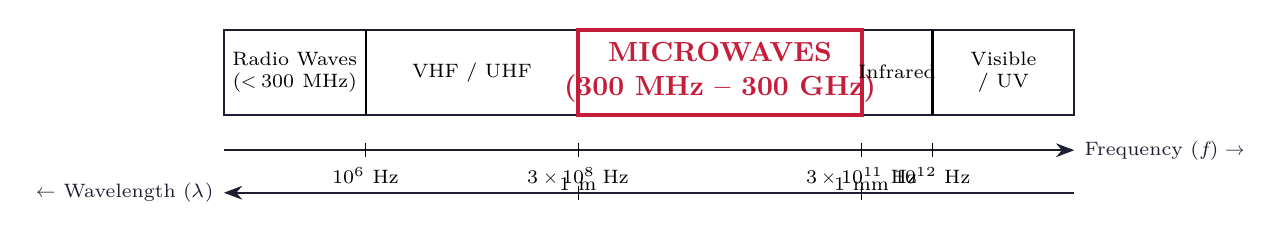
\begin{tikzpicture}[scale=0.9, every node/.style={font=\scriptsize}]
  % Draw spectrum bar
  \draw[thick, color=mydark] (0,0) rectangle (12,1.2);
  
  % Dividers and Labels
  \draw[thick] (2,0) -- (2,1.2);
  \draw[thick] (5,0) -- (5,1.2);
  \draw[thick, color=myred, line width=1.5pt] (5,0) rectangle (9,1.2);
  \draw[thick] (10,0) -- (10,1.2);
  
  \node[align=center] at (1,0.6) {Radio Waves\\($<300$ MHz)};
  \node[align=center, font=\bfseries\color{myred}] at (7,0.6) {MICROWAVES\\(300 MHz -- 300 GHz)};
  \node at (3.5,0.6) {VHF / UHF};
  \node at (9.5,0.6) {Infrared};
  \node[align=center] at (11,0.6) {Visible\\/ UV};
  
  % Frequency and Wavelength axis markers below
  \draw[arrow] (0,-0.5) -- (12,-0.5) node[right] {Frequency ($f$) $\to$};
  \draw[arrow] (12,-1.1) -- (0,-1.1) node[left] {$\gets$ Wavelength ($\lambda$)};
  
  % Ticks for frequency
  \draw (2,-0.4) -- (2,-0.6) node[below] {$10^6$ Hz};
  \draw (5,-0.4) -- (5,-0.6) node[below] {$3 \times 10^8$ Hz};
  \draw (9,-0.4) -- (9,-0.6) node[below] {$3 \times 10^{11}$ Hz};
  \draw (10,-0.4) -- (10,-0.6) node[below] {$10^{12}$ Hz};
  
  % Ticks for wavelength
  \draw (5,-1.0) -- (5,-1.2) node[above] {$1$ m};
  \draw (9,-1.0) -- (9,-1.2) node[above] {$1$ mm};
\end{tikzpicture}
\tcbset{colbacktitle=myteal, coltitle=white}
\end{tcolorbox}

% ===============================================================================
\section{Microwave Frequency Bands}
% ===============================================================================

To avoid spectral confusion, the microwave spectrum is subdivided into distinct bands. The two primary naming standards are the \textbf{IEEE Standard} (used in radar and communications) and the \textbf{Military/NATO Standard}.

\subsection{IEEE Microwave Frequency Band Classification}
The table below details the frequency and wavelength ranges defined by the IEEE:

\par\noindent
{\renewcommand{\arraystretch}{1.55}%
\begin{tabularx}{\linewidth}{|B{3.2cm}|Y|Y|Y|}\hline
\textbf{Band Designation} & \textbf{Frequency Range} & \textbf{Wavelength Range} & \textbf{Typical Applications} \\[4pt]
\hline
\textbf{L Band} & $1.0 - 2.0$ GHz & $30.0 - 15.0$ cm & GPS, Mobile phones (GSM), Satellite navigation \\[4pt]
\hline
\textbf{S Band} & $2.0 - 4.0$ GHz & $15.0 - 7.5$ cm & Wi-Fi (2.4 GHz), Microwave ovens, Weather radars \\[4pt]
\hline
\textbf{C Band} & $4.0 - 8.0$ GHz & $7.5 - 3.75$ cm & Satellite TV transponders, Wi-Fi (5.8 GHz) \\
\hline
\textbf{X Band} & $8.0 - 12.0$ GHz & $3.75 - 2.50$ cm & Military radar, Marine navigation, Speed detectors \\[4pt]
\hline
\textbf{Ku Band} & $12.0 - 18.0$ GHz & $2.50 - 1.67$ cm & Direct-to-Home (DTH) TV, Satellite networks \\[4pt]
\hline
\textbf{K Band} & $18.0 - 27.0$ GHz & $1.67 - 1.11$ cm & Radar altimeters, Water vapour absorption line (22 GHz) \\[4pt]
\hline
\textbf{Ka Band} & $27.0 - 40.0$ GHz & $1.11 - 0.75$ cm & High-speed satellite broadband, Close-range radar \\[4pt]
\hline
\textbf{V Band} & $40.0 - 75.0$ GHz & $7.5 - 4.0$ mm & Short-range military comms, 60 GHz Wi-Fi (IEEE 802.11ad) \\[4pt]
\hline
\textbf{W Band} & $75.0 - 110$ GHz & $4.0 - 2.7$ mm & Automotive radars, Millimeter-wave imaging \\
\hline
\end{tabularx}
}

% ===============================================================================
\section{Key Advantages and Properties of Microwaves}
% ===============================================================================

Microwaves possess specific properties that differentiate them from lower-frequency radio waves:

\begin{enumerate}[label=\textbf{\arabic*.}, leftmargin=*, itemsep=4pt]
  \item \textbf{High Information Carrying Capacity (Large Bandwidth):} The available bandwidth in the microwave region is several orders of magnitude larger than the entire HF and VHF radio spectrum combined.
    \begin{equation}
      \text{Bandwidth } \Delta f = f_2 - f_1
    \end{equation}
    Since frequency is high, a small fractional bandwidth yields enormous absolute bandwidth, enabling high-rate data transmission.
  \item \textbf{Line-of-Sight (LoS) Propagation:} Microwaves travel in straight lines and are not reflected by the ionosphere. This ensures clean, interference-free point-to-point communication but requires repeater towers due to earth's curvature.
  \item \textbf{Directive Antenna Gain:} The gain of an antenna is inversely proportional to the square of the wavelength:
    \begin{equation}
      G = \frac{4\pi A_e}{\lambda^2}
    \end{equation}
    Because $\lambda$ is small, very high antenna gain and narrow beamwidths can be achieved with physically small structures (e.g., dish antennas).
  \item \textbf{Lower Power Requirements:} Highly directive antennas concentrate energy into a narrow beam, requiring significantly lower transmitter power to span long links compared to omnidirectional HF systems.
  \item \textbf{Ionospheric Transparency:} Frequencies above 100 MHz pass directly through the ionosphere without being reflected or bent, making space, satellite, and deep-space communications possible.
\end{enumerate}

% ===============================================================================
\section{Applications of Microwaves}
% ===============================================================================

\subsection{Civil and Military Applications}
The primary applications of microwaves are split across the civilian and defense sectors:

\textbf{Civilian Applications:}
\begin{itemize}[leftmargin=*, itemsep=2pt]
  \item \textbf{Telecommunications:} Cellular networks (LTE, 5G), Wi-Fi router bands, and satellite voice/data networks.
  \item \textbf{Satellite Broadcasting:} Direct-to-Home (DTH) TV services (operating in the Ku band) and satellite radio.
  \item \textbf{Meteorology:} Weather radar systems operating in the S and C bands to map precipitation and storm tracks.
  \item \textbf{Domestic Heating:} Microwave ovens operate at 2.45 GHz, utilizing dielectric heating of water molecules in food.
\end{itemize}

\textbf{Military Applications:}
\begin{itemize}[leftmargin=*, itemsep=2pt]
  \item \textbf{Radar Detection and Tracking:} Fire-control radars, air traffic monitoring, and target tracking (operating in X and Ku bands).
  \item \textbf{Electronic Warfare (EW):} Jamming enemy communications, electronic countermeasures (ECM), and radar signature reduction (stealth).
  \item \textbf{Missile Guidance:} Semi-active and active radar seekers located in the nose cones of missiles.
\end{itemize}

\subsection{Medical Applications}
Microwaves interact with biological tissues in ways that enable both diagnostics and therapy:
\begin{itemize}[leftmargin=*, itemsep=3pt]
  \item \textbf{Microwave Hyperthermia:} Delivering controlled heat to tumors. Cancer cells are more heat-sensitive than healthy tissue, and raising their temperature to $42^\circ\text{C}$--$45^\circ\text{C}$ helps destroy them.
  \item \textbf{Microwave Ablation (MWA):} Using localized needle-like microwave antennas inserted into tumors to cook and destroy cancer cells directly.
  \item \textbf{Microwave Imaging:} Utilizing dielectric contrast between healthy and malignant breast tissues to detect tumors without ionizing radiation.
\end{itemize}

% ===============================================================================
\section{EMI/EMC Concepts at Microwave Frequencies}
% ===============================================================================

As operating frequencies increase, electromagnetic interactions become critical, necessitating strict EMI/EMC compliance.

\begin{tcolorbox}[defbox]
\textbf{EMI (Electromagnetic Interference):} Any electromagnetic disturbance or emission that degrades, disrupts, or limits the effective performance of electrical equipment.

\textbf{EMC (Electromagnetic Compatibility):} The ability of an electrical system or device to function satisfactorily in its electromagnetic environment without introducing intolerable electromagnetic disturbances to anything in that environment.
\end{tcolorbox}

\subsection{The EMI Coupling Path}
For electromagnetic interference to occur, three elements must be present:

\begin{tcolorbox}[tikzbox, title={Elements of Electromagnetic Interference}]
\centering
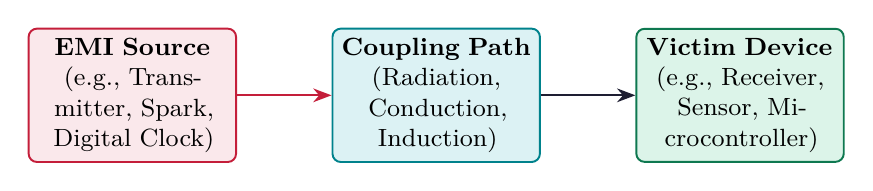
\begin{tikzpicture}[node distance=0.6cm and 1.2cm]
  \node[redblock] (src) {\textbf{EMI Source}\\(e.g., Transmitter, Spark, Digital Clock)};
  \node[block, right=1.2cm of src] (path) {\textbf{Coupling Path}\\(Radiation, Conduction, Induction)};
  \node[block, draw=mygreen, fill=hdrgreen, right=1.2cm of path] (vic) {\textbf{Victim Device}\\(e.g., Receiver, Sensor, Microcontroller)};
  
  \draw[arrow, color=myred] (src) -- (path);
  \draw[arrow] (path) -- (vic);
\end{tikzpicture}
\end{tcolorbox}

\subsection{EMI Mitigation Techniques}
\begin{itemize}[leftmargin=*, itemsep=2pt]
  \item \textbf{Shielding:} Enclosing sensitive circuits in metallic containers (Faraday cages) to reflect and absorb radiated fields.
  \item \textbf{Grounding:} Ensuring low-impedance ground return paths to prevent common-mode voltage differences.
  \item \textbf{Filtering:} Installing low-pass filters on power and signal lines to suppress high-frequency noise.
\end{itemize}

% ===============================================================================
% MANDATORY QUICK REVISION PAGE
% ===============================================================================
\newpage
\begin{center}
  {\large\bfseries\color{myred} Quick Revision --- Module I}\\[3pt]
  {\small\color{mydark} Introduction to Microwaves $|$ PE-EC701A}
\end{center}
\noindent{\color{myred}\rule{\linewidth}{1.2pt}}
\vspace{4pt}

\begin{tcolorbox}[formulabox, title={\textbf{Key Formulas at a Glance}}]
\renewcommand{\arraystretch}{1.3}
\begin{tabularx}{\linewidth}{B{4.5cm} X}Wave Velocity Relation  & $c = f \lambda \approx 3 \times 10^8 \text{ m/s}$ (in free space) \\[4pt]
Antenna Directivity/Gain & $G = \frac{4\pi A_e}{\lambda^2}$ \quad ($A_e$ = effective aperture area) \\[4pt]
Bandwidth               & $\Delta f = f_2 - f_1$ \\[4pt]
Decibel Power Ratio     & $P_{\text{dB}} = 10 \log_{10}\left(\frac{P_{\text{out}}}{P_{\text{in}}}\right)$
\end{tabularx}
\end{tcolorbox}

\begin{tcolorbox}[defbox, title={\textbf{One-Line Definitions}}]
\begin{itemize}[leftmargin=*, itemsep=2.5pt, topsep=0pt]
  \item \textbf{Microwave:} Electromagnetic waves operating between 300 MHz and 300 GHz.
  \item \textbf{Dominant Mode:} The waveguide transmission mode that exhibits the lowest cutoff frequency.
  \item \textbf{Line-of-Sight:} Straight-line propagation between antennas with no ionospheric reflection.
  \item \textbf{EMI:} Disturbance of electronic systems caused by unintended electromagnetic fields.
  \item \textbf{EMC:} The capacity of a device to operate without radiating or absorbing excessive EMI.
  \item \textbf{Microwave Hyperthermia:} Thermal therapy utilizing microwaves to selectively heat and destroy tumor cells.
  \item \textbf{Faraday Cage:} A conductive enclosure used to block external radiated electromagnetic fields.
\end{itemize}
\end{tcolorbox}

\begin{tcolorbox}[exambox, title={\textbf{Frequently Asked / Viva Questions}}]
\begin{enumerate}[topsep=0pt, label=\textbf{Q\arabic*.}, itemsep=5pt]
  \item \Q{State the frequency and wavelength ranges of microwaves.}
    Frequencies range from 300 MHz to 300 GHz, corresponding to free-space wavelengths of 1 m to 1 mm respectively.
  \item \Q{Why are microwaves not reflected by the ionosphere?}
    Because of their high frequencies ($>100$ MHz). The ionospheric plasma frequency is lower, allowing microwaves to pass directly through without reflection.
  \item \Q{What are the typical frequency ranges for the L, S, C, and X bands?}
    L band: $1 - 2$ GHz; S band: $2 - 4$ GHz; C band: $4 - 8$ GHz; X band: $8 - 12$ GHz.
  \item \Q{Why are microwave antennas physically small for a given high gain?}
    Gain is inversely proportional to $\lambda^2$ ($G = 4\pi A_e/\lambda^2$). Since $\lambda$ is small, a small aperture $A_e$ is sufficient to achieve high gain.
  \item \Q{List three major advantages of using microwaves for communication.}
    Large operational bandwidth (high information capacity), high antenna directivity, and immunity to ionospheric disturbances.
  \item \Q{What is the operating frequency of a domestic microwave oven and why?}
    2.45 GHz. This frequency matches the rotational excitation energy of water molecules, ensuring efficient dielectric heating of food.
  \item \Q{Explain the difference between EMI and EMC.}
    EMI is the interference signal itself that disrupts electronic operation. EMC is the design property of a system to resist EMI and avoid emitting it.
  \item \Q{State the medical applications of microwaves.}
    Microwave hyperthermia for cancer therapy, microwave ablation to destroy tissue, and non-invasive microwave breast imaging.
  \item \Q{Why is point-to-point microwave communication limited by distance?}
    Because microwaves propagate in straight lines (LoS). Due to the earth's curvature, repeater stations are required approximately every 50 km.
  \item \Q{What is the significance of the X-band in military applications?}
    X-band ($8 - 12$ GHz) offers a good compromise between atmospheric attenuation and spatial resolution, making it ideal for tracking and fire-control radars.
  \item \Q{How does high operating frequency affect digital circuits regarding EMI?}
    As frequency increases, trace lines on PCBs act as antennas, leading to crosstalk, radiation emission, and high susceptibility to noise.
  \item \Q{What is shielding effectiveness (SE)?}
    It is the ratio of the electromagnetic field strength before shielding to the field strength after shielding, measured in decibels (dB).
\end{enumerate}
\end{tcolorbox}

\begin{tcolorbox}[tikzbox, title={Comparison of Civil and Military Microwave Applications}]
\renewcommand{\arraystretch}{1.4}
\par\noindent
{\renewcommand{\arraystretch}{1.55}%
\begin{tabularx}{\linewidth}{|B{3.0cm}|Y|Y|}\hline
\textbf{Parameter} & \textbf{\color{myteal}Civil Applications} & \textbf{\color{myred}Military Applications} \\[4pt]
\hline
\textbf{Primary Goal} & High-capacity data transfer, media broadcast, and domestic heating. & Surveillance, threat tracking, weapons guidance, and communications jamming. \\[4pt]
\hline
\textbf{Typical Bands} & L, S, C, Ku bands (high-speed data, DTH satellite). & X, Ku, Ka, W bands (fine-resolution radar, stealth systems). \\[4pt]
\hline
\textbf{Design Priority} & Cost efficiency, standardized channels, and regulatory compliance. & High reliability, anti-jamming capabilities, and high-power output. \\[4pt]
\hline
\textbf{Standard Devices} & Solid-state transceivers, standard Wi-Fi routers. & High-power magnetrons, traveling-wave tubes (TWT), and phased-array systems. \\[4pt]
\hline
\end{tabularx}
}
\end{tcolorbox}


% -- Module 2 -----------------------------------------------------------------
\modulestart{2}{Concept of Wave Modes}

\section{Concept of Wave Modes}
% ===============================================================================

When electromagnetic waves propagate along a guide structure, the boundaries dictate how the fields are oriented. These field distributions are classified as modes.

\begin{tcolorbox}[defbox]
\textbf{Wave Mode:} A specific configuration of electric and magnetic fields that satisfies Maxwell's equations and the boundary conditions of the transmission structure. Modes are characterized by their cutoff frequencies and spatial patterns.
\end{tcolorbox}

\subsection{Classification of Modes}
We classify electromagnetic modes based on the presence of longitudinal field components along the direction of propagation (assumed to be the $z$-axis):
\begin{itemize}[leftmargin=*, itemsep=3pt]
  \item \textbf{TEM (Transverse Electromagnetic) Mode:}
    Both the electric and magnetic fields are entirely transverse to the direction of propagation.
    \begin{equation}
      E_z = 0 \quad \text{and} \quad H_z = 0
    \end{equation}
  \item \textbf{TE (Transverse Electric) Mode:}
    The electric field is completely transverse to the direction of propagation, while the magnetic field has a longitudinal component.
    \begin{equation}
      E_z = 0 \quad \text{and} \quad H_z \ne 0
    \end{equation}
  \item \textbf{TM (Transverse Magnetic) Mode:}
    The magnetic field is completely transverse to the direction of propagation, while the electric field has a longitudinal component.
    \begin{equation}
      H_z = 0 \quad \text{and} \quad E_z \ne 0
    \end{equation}
  \item \textbf{Hybrid Modes (HE/EH):}
    Both electric and magnetic fields have non-zero longitudinal components.
    \begin{equation}
      E_z \ne 0 \quad \text{and} \quad H_z \ne 0
    \end{equation}
\end{itemize}

\subsection{Field Lines in Waveguide Cross-Sections}
The physical layout of the electric ($\vec{E}$) and magnetic ($\vec{H}$) fields is visualized below:

\begin{tcolorbox}[tikzbox, title={Field Distribution in Coaxial (TEM) and Rectangular Waveguide ($\text{TE}_{10}$)}]
\centering
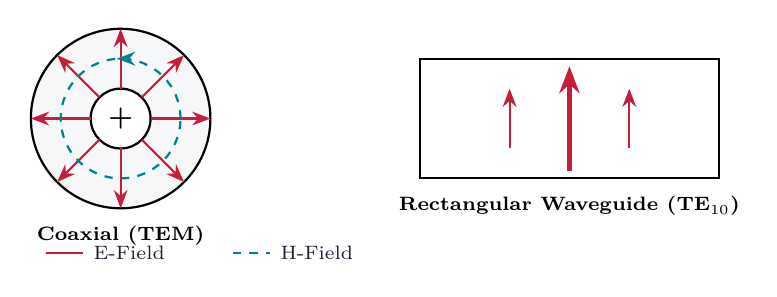
\begin{tikzpicture}[scale=0.95]
  % Coaxial (TEM)
  \draw[thick, fill=mygray] (-3,0) circle (1.2cm);
  \draw[thick, fill=white] (-3,0) circle (0.4cm);
  \node[font=\bfseries] at (-3,0) {+};
  \node[below, font=\scriptsize\bfseries] at (-3,-1.3) {Coaxial (TEM)};
  
  % Radial E-field lines
  \foreach \angle in {0, 45, 90, 135, 180, 225, 270, 315} {
    \draw[-Stealth, color=myred, thick] (-3,0) +(\angle:0.4) -- +(\angle:1.2);
  }
  % Concentric H-field lines
  \draw[dashed, color=myteal, thick] (-3,0) circle (0.8cm);
  \draw[-Stealth, color=myteal, thick] (-3,0.8) -- (-3.05,0.8);
  
  % Rectangular Waveguide (TE10)
  \draw[thick] (1,-0.8) rectangle (5,0.8);
  \node[below, font=\scriptsize\bfseries] at (3,-0.9) {Rectangular Waveguide ($\text{TE}_{10}$)};
  
  % E-field vertical lines (sinusoidal profile in center)
  \draw[-Stealth, color=myred, thick] (2.2,-0.4) -- (2.2,0.4);
  \draw[-Stealth, color=myred, line width=1.5pt] (3.0,-0.7) -- (3.0,0.7);
  \draw[-Stealth, color=myred, thick] (3.8,-0.4) -- (3.8,0.4);
  
  % H-field closed loops (represented in cross section as points/crosses or loops)
  % Show E-field legend
  \draw[thick, color=myred] (-4,-1.8) -- (-3.5,-1.8) node[right, font=\scriptsize, color=mydark] {E-Field};
  \draw[dashed, thick, color=myteal] (-1.5,-1.8) -- (-1.0,-1.8) node[right, font=\scriptsize, color=mydark] {H-Field};
\end{tikzpicture}
\end{tcolorbox}

% ===============================================================================
\section{Proof of Non-Existence of TEM Mode in Hollow Waveguides}
% ===============================================================================

A central mathematical model shows that TEM waves cannot propagate inside single-conductor hollow waveguides.

\begin{tcolorbox}[defbox, title={\textbf{Theorem}}]
TEM waves cannot exist inside a hollow waveguide formed by a single closed conductor. They require at least two distinct conductors (e.g., coaxial line) to propagate.
\end{tcolorbox}

\subsubsection{Mathematical Proof}
Assume a TEM wave propagates along the $z$-direction in a hollow waveguide with a single conductor wall $C$. For a TEM mode, by definition:
\begin{equation*}
  E_z = 0 \quad \text{and} \quad H_z = 0
\end{equation*}
From Maxwell's curl equation for the electric field:
\begin{equation*}
  \nabla \times \vec{E} = -j\omega\mu \vec{H}
\end{equation*}
Analyzing the $z$-component of the curl:
\begin{equation}
  \frac{\partial E_y}{\partial x} - \frac{\partial E_x}{\partial y} = -j\omega\mu H_z
\end{equation}
Since $H_z = 0$, this yields:
\begin{equation}
  \frac{\partial E_y}{\partial x} - \frac{\partial E_x}{\partial y} = 0
\end{equation}
This indicates that the transverse electric field $\vec{E}_t = E_x \hat{a}_x + E_y \hat{a}_y$ has a curl of zero in the transverse plane. Therefore, the transverse electric field can be expressed as the gradient of a scalar electrostatic potential function $\Phi(x, y)$:
\begin{equation}
  \vec{E}_t = -\nabla_t \Phi(x, y)
\end{equation}
Next, we invoke Gauss's Law in the charge-free dielectric region inside the waveguide:
\begin{equation*}
  \nabla \cdot \vec{E} = 0 \implies \frac{\partial E_x}{\partial x} + \frac{\partial E_y}{\partial y} + \frac{\partial E_z}{\partial z} = 0
\end{equation*}
Since $E_z = 0$, the divergence equation reduces to the transverse plane:
\begin{equation}
  \nabla_t \cdot \vec{E}_t = 0
\end{equation}
Substituting $\vec{E}_t = -\nabla_t \Phi$ into the divergence equation yields:
\begin{equation}
  \nabla_t^2 \Phi(x, y) = 0 \quad (\text{Laplace's Equation})
\end{equation}
Now we apply the boundary conditions on the waveguide boundary $C$. Since the wall is a Perfect Electric Conductor (PEC), the tangential electric field must vanish on $C$.
This implies the conductor boundary is an equipotential surface:
\begin{equation}
  \Phi(x, y) = \Phi_0 \quad (\text{constant}) \quad \text{on boundary } C
\end{equation}
According to the \textbf{uniqueness theorem} of Laplace's equation:
If a potential $\Phi$ satisfies Laplace's equation ($\nabla^2 \Phi = 0$) within a closed region bounded by a single conductor at a constant potential $\Phi_0$, then the potential must be constant everywhere inside that region:
\begin{equation}
  \Phi(x, y) = \Phi_0 \quad \text{for all } x, y \text{ inside } C
\end{equation}
Taking the gradient of a constant potential to find the electric field:
\begin{equation}
  \vec{E}_t = -\nabla_t \Phi_0 = 0
\end{equation}
If the electric field is zero everywhere inside the waveguide, then by Maxwell's equations, the magnetic field is also zero:
\begin{equation}
  \vec{H}_t = 0
\end{equation}
Thus, no electromagnetic fields can exist inside the guide. Therefore, \textbf{TEM modes cannot exist inside a hollow, single-conductor waveguide} (Q.E.D.).

% ===============================================================================
\section{Losses Associated with Microwave Transmission}
% ===============================================================================

Energy propagating down a microwave line attenuates due to three primary physical loss mechanisms:

\subsection{Conductor Losses (Skin Effect)}
At microwave frequencies, current does not distribute uniformly across the conductor cross-section but crowds near the surface.
\begin{tcolorbox}[defbox]
\textbf{Skin Depth ($\delta$):} The depth into a conductor at which the electromagnetic wave amplitude decays to $1/e$ (approx. $36.8\%$) of its surface value.
\end{tcolorbox}

\begin{tcolorbox}[formulabox, title={\textbf{Skin Depth and Surface Resistance}}]
The skin depth $\delta$ is given by:
\begin{equation}
  \delta = \frac{1}{\sqrt{\pi f \mu \sigma}} \quad (\text{m})
\end{equation}
The corresponding surface resistance $R_s$ is:
\begin{equation}
  R_s = \frac{1}{\sigma \delta} = \sqrt{\frac{\pi f \mu}{\sigma}} \quad (\Omega/\text{square})
\end{equation}
Where:
\begin{itemize}[leftmargin=1.5em, itemsep=1pt, topsep=2pt]
  \item[] $f$ = frequency of operation (Hz)
  \item[] $\mu$ = permeability of the conductor ($\text{H/m}$)
  \item[] $\sigma$ = conductivity of the metal ($\text{S/m}$)
\end{itemize}
\end{tcolorbox}

\subsection{Dielectric Losses}
Dielectric losses occur in the medium filling the waveguide due to the rotation of polar molecules under high-frequency alternating electric fields. It is quantified using the loss tangent ($\tan \delta$):
\begin{equation}
  \alpha_d = \frac{\omega \epsilon''}{2 \beta} \approx \frac{\pi \sqrt{\epsilon_r} \tan \delta}{\lambda_0} \quad (\text{Np/m})
\end{equation}

\subsection{Radiation Losses}
Radiation losses occur primarily in open-boundary lines (e.g., Microstrip lines) where fields are not completely enclosed, allowing some energy to radiate outward as radio waves.

% ===============================================================================
\section{Concept of Wave Impedance}
% ===============================================================================

\begin{tcolorbox}[defbox]
\textbf{Wave Impedance ($Z_w$):} The ratio of the transverse electric field to the transverse magnetic field for a propagating mode. It represents the characteristic resistance that the wave encounters as it travels.
\end{tcolorbox}

The wave impedance depends heavily on the mode type (TE or TM) and the operating frequency:

\begin{tcolorbox}[formulabox, title={\textbf{Wave Impedance Formulations}}]
Let $\eta = \sqrt{\mu/\epsilon}$ be the intrinsic impedance of the dielectric medium. The wave impedances for TE and TM modes are:
\begin{align}
  Z_{\text{TE}} &= \frac{\eta}{\sqrt{1 - \left(\frac{f_c}{f}\right)^{\!2}}} \quad (\Omega) \\
  Z_{\text{TM}} &= \eta \sqrt{1 - \left(\frac{f_c}{f}\right)^{\!2}} \quad (\Omega)
\end{align}
Where:
\begin{itemize}[leftmargin=1.5em, itemsep=1pt, topsep=2pt]
  \item[] $f_c$ = Cutoff frequency of the specific mode
  \item[] $f$ = Operating frequency
\end{itemize}
\textbf{Critical Limits:}
\begin{itemize}[leftmargin=1.5em, itemsep=1pt]
  \item For $f < f_c$ (below cutoff): Impedance is purely imaginary, indicating evanescent (non-propagating) fields.
  \item For $f \to \infty$: Both $Z_{\text{TE}}$ and $Z_{\text{TM}}$ approach the intrinsic impedance $\eta$ of the medium.
\end{itemize}
\end{tcolorbox}

% ===============================================================================
% MANDATORY QUICK REVISION PAGE
% ===============================================================================
\newpage
\begin{center}
  {\large\bfseries\color{myred} Quick Revision --- Module II}\\[3pt]
  {\small\color{mydark} Mathematical Model of Microwave Transmission $|$ PE-EC701A}
\end{center}
\noindent{\color{myred}\rule{\linewidth}{1.2pt}}
\vspace{4pt}

\begin{tcolorbox}[formulabox, title={\textbf{Key Formulas at a Glance}}]
\renewcommand{\arraystretch}{1.3}
\begin{tabularx}{\linewidth}{B{4.5cm} X}Skin Depth              & $\delta = \frac{1}{\sqrt{\pi f \mu \sigma}}$ \\[4pt]
Surface Resistance      & $R_s = \sqrt{\frac{\pi f \mu}{\sigma}}$ \\[4pt]
TE Wave Impedance       & $Z_{\text{TE}} = \frac{\eta}{\sqrt{1 - (f_c/f)^2}}$ \\[4pt]
TM Wave Impedance       & $Z_{\text{TM}} = \eta \sqrt{1 - (f_c/f)^2}$ \\[4pt]
Intrinsic Impedance     & $\eta = \sqrt{\frac{\mu}{\epsilon}} \approx 377\,\Omega$ (in free space)
\end{tabularx}
\end{tcolorbox}

\begin{tcolorbox}[defbox, title={\textbf{One-Line Definitions}}]
\begin{itemize}[leftmargin=*, itemsep=2.5pt, topsep=0pt]
  \item \textbf{Wave Mode:} A valid mathematical field pattern satisfying boundary conditions.
  \item \textbf{TEM Mode:} A mode with zero electric and magnetic fields in the direction of propagation.
  \item \textbf{Wave Impedance:} The ratio of transverse electric field to transverse magnetic field.
  \item \textbf{Skin Depth:} The distance in a metal where current density drops to $36.8\%$ of surface value.
  \item \textbf{Uniqueness Theorem:} Electrostatic theorem proving Laplace's solution is unique under boundary limits.
  \item \textbf{Evanescent Wave:} An attenuated wave that does not carry real power, occurring below cutoff.
  \item \textbf{Loss Tangent:} A measure of energy dissipation in a lossy dielectric material.
\end{itemize}
\end{tcolorbox}

\begin{tcolorbox}[exambox, title={\textbf{Frequently Asked / Viva Questions}}]
\begin{enumerate}[topsep=0pt, label=\textbf{Q\arabic*.}, itemsep=5pt]
  \item \Q{Why can TEM waves not exist inside a hollow waveguide?}
    Because the waveguide wall is a single conductor that acts as an equipotential boundary. Inside, Laplace's equation forces the potential to be constant, making the electric fields zero.
  \item \Q{What transmission structures support TEM waves?}
    Structures with two or more isolated conductors, such as coaxial lines, striplines, and microstrip lines.
  \item \Q{How does skin depth vary with frequency?}
    It is inversely proportional to the square root of frequency ($\delta \propto 1/\sqrt{f}$). Higher frequencies yield thinner skin depths.
  \item \Q{Why do conductor losses increase at microwave frequencies?}
    Because current is confined to a very thin layer (skin depth), effectively reducing the cross-sectional area of conduction and increasing resistance.
  \item \Q{Explain the behaviour of $Z_{\text{TE}}$ as frequency approaches the cutoff frequency $f_c$ from above.}
    As $f \to f_c^+$, the denominator $\sqrt{1-(f_c/f)^2} \to 0$, causing the wave impedance $Z_{\text{TE}}$ to approach infinity.
  \item \Q{What happens to the wave impedance of a TM mode below cutoff ($f < f_c$)?}
    The term inside the radical becomes negative, making the wave impedance purely reactive/imaginary, indicating no real power propagation.
  \item \Q{What is the physical significance of the loss tangent ($\tan \delta$)?}
    It represents the ratio of the lossy conduction current density to the lossless displacement current density in a dielectric.
  \item \Q{Why do we use copper or silver plating inside microwave guides?}
    To reduce conductor losses. Since currents flow within a few microns of the surface, a thin layer of highly conductive material reduces surface resistance $R_s$.
  \item \Q{State the intrinsic impedance of free space.}
    $\eta_0 = \sqrt{\mu_0/\epsilon_0} \approx 120\pi \approx 377\,\Omega$.
  \item \Q{What is the difference between TE and TM modes?}
    In TE modes, the longitudinal electric field is zero ($E_z = 0, H_z \ne 0$). In TM modes, the longitudinal magnetic field is zero ($H_z = 0, E_z \ne 0$).
  \item \Q{How does the cutoff frequency affect mode propagation?}
    Waves only propagate if their operating frequency exceeds the cutoff frequency ($f > f_c$). Below cutoff, waves decay exponentially.
  \item \Q{What are hybrid modes?}
    Modes where both the longitudinal electric and magnetic fields are non-zero ($E_z \ne 0$ and $H_z \ne 0$). They are common in optical fibers.
\end{enumerate}
\tcbset{colbacktitle=mgframe, coltitle=mydark}
\end{tcolorbox}

\begin{tcolorbox}[tikzbox, title={Comparison of Wave Propagation Modes}]
\renewcommand{\arraystretch}{1.4}
\par\noindent
{\renewcommand{\arraystretch}{1.9}%
\begin{tabularx}{\linewidth}{|B{3.2cm}|Y|Y|Y|}\hline
\textbf{Feature} & \textbf{TEM Mode} & \textbf{TE Mode} & \textbf{TM Mode} \\
\hline
\textbf{Longitudinal $E_z$} & $E_z = 0$ & $E_z = 0$ & $E_z \ne 0$ \\[4pt]
\hline
\textbf{Longitudinal $H_z$} & $H_z = 0$ & $H_z \ne 0$ & $H_z = 0$ \\[4pt]
\hline
\textbf{Hollow Guide?} & No & Yes & Yes \\
\hline
\textbf{Wave Impedance} & $Z_w = \eta$ & $Z_w = \eta / \sqrt{1-(f_c/f)^2}$ & $Z_w = \eta \sqrt{1-(f_c/f)^2}$ \\[6pt]
\hline
\textbf{Cutoff Freq $f_c$} & $f_c = 0$ & $f_c > 0$ & $f_c > 0$ \\[4pt]
\hline
\end{tabularx}
}
\end{tcolorbox}


% -- Module 3 -----------------------------------------------------------------
\modulestart{3}{Coaxial Line}

\section{Coaxial Line}
% ===============================================================================

The coaxial line is a standard TEM transmission line with two concentric circular conductors. It operates from DC up to frequencies where higher-order waveguide modes (usually $\text{TE}_{11}$) begin to propagate.

\begin{tcolorbox}[tikzbox, title={Coaxial Line Structure}]
\begin{minipage}[c]{0.45\linewidth}
\centering
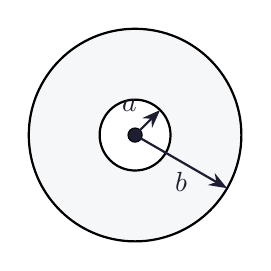
\begin{tikzpicture}[scale=0.9]
  \draw[thick, fill=mygray] (0,0) circle (1.5cm);
  \draw[thick, fill=white] (0,0) circle (0.5cm);
  \draw[fill=mydark] (0,0) circle (0.1cm);
  
  \draw[arrow] (0,0) -- (45:0.5) node[midway, above left] {$a$};
  \draw[arrow] (0,0) -- (-30:1.5) node[midway, below] {$b$};
\end{tikzpicture}
\end{minipage}\hfill
\begin{minipage}[c]{0.5\linewidth}
\raggedright
\textbf{Conductors:}\\[3pt]
Inner Radius = $a$\\
Outer Radius = $b$\\
Dielectric constant = $\epsilon_r$
\end{minipage}
\end{tcolorbox}

\begin{tcolorbox}[formulabox, title={\textbf{Coaxial Line Characteristic Impedance}}]
The characteristic impedance $Z_0$ of a lossless coaxial line is given by:
\begin{equation}
  Z_0 = \frac{\eta_0}{2\pi \sqrt{\epsilon_r}} \ln\left(\frac{b}{a}\right) \approx \frac{138}{\sqrt{\epsilon_r}} \log_{10}\left(\frac{b}{a}\right) \quad (\Omega)
\end{equation}
Where:
\begin{itemize}[leftmargin=1.5em, itemsep=1pt, topsep=2pt]
  \item[] $\eta_0 \approx 377\,\Omega$ is the intrinsic impedance of free space.
  \item[] $\epsilon_r$ is the relative permittivity of the dielectric.
\end{itemize}
\end{tcolorbox}

% ===============================================================================
\section{Rectangular Waveguide}
% ===============================================================================

A rectangular waveguide is a hollow metallic pipe of rectangular cross-section. Since it has only one conductor, it cannot support TEM waves; propagation occurs via TE and TM modes.

\begin{tcolorbox}[tikzbox, title={Rectangular Waveguide Geometry}]
\begin{minipage}[c]{0.52\linewidth}
\centering
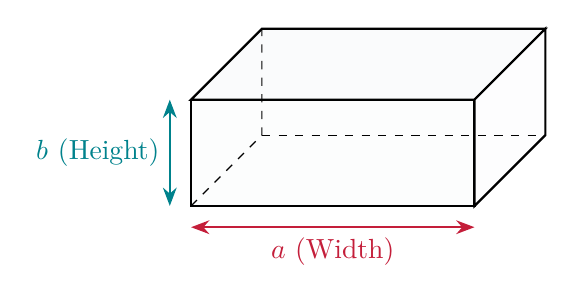
\begin{tikzpicture}[scale=0.9]
  % Draw 3D-like rectangular waveguide
  \draw[thick, fill=mygray!50] (0,0) -- (4,0) -- (5,1) -- (1,1) -- cycle;
  \draw[thick, fill=mygray!30] (0,-1.5) -- (4,-1.5) -- (4,0) -- (0,0) -- cycle;
  \draw[thick, fill=mygray!20] (4,-1.5) -- (5,-0.5) -- (5,1) -- (4,0) -- cycle;
  
  % Inner dotted lines for back boundaries
  \draw[dashed] (0,-1.5) -- (1,-0.5) -- (1,1);
  \draw[dashed] (1,-0.5) -- (5,-0.5);
  
  % Dimension indicators
  \draw[Stealth-Stealth, thick, color=myred] (0,-1.8) -- (4,-1.8) node[midway, below] {$a$ (Width)};
  \draw[Stealth-Stealth, thick, color=myteal] (-0.3,-1.5) -- (-0.3,0) node[midway, left] {$b$ (Height)};
\end{tikzpicture}
\end{minipage}\hfill
\begin{minipage}[c]{0.43\linewidth}
\raggedright
\textbf{Dominant dimension relation:}\\[3pt]
$a > b$\\[2pt]
Typically, $a = 2b$ to maximize single-mode bandwidth.
\end{minipage}
\end{tcolorbox}

\subsection{Wave Equations and Mode Cutoff}
From Helmholtz wave equations inside a lossless rectangular guide:
\begin{equation}
  f_c = \frac{v_0}{2} \sqrt{\left(\frac{m}{a}\right)^{\!2} + \left(\frac{n}{b}\right)^{\!2}} = \frac{c}{2\sqrt{\epsilon_r}} \sqrt{\left(\frac{m}{a}\right)^{\!2} + \left(\frac{n}{b}\right)^{\!2}}
\end{equation}
Where $m$ and $n$ are mode integers. The \textbf{dominant mode} (lowest cutoff frequency) for $a > b$ is the \textbf{$\text{TE}_{10}$ mode} ($m=1, n=0$):
\begin{equation}
  f_{c(\text{TE}_{10})} = \frac{c}{2a\sqrt{\epsilon_r}}
\end{equation}

\subsection{Phase Velocity, Group Velocity, and Guide Wavelength}
Waveguide propagation constants vary non-linearly with frequency:
\begin{itemize}[leftmargin=*, itemsep=3pt]
  \item \textbf{Guide Wavelength ($\lambda_g$):} The distance between two equal-phase planes along the guide axis.
    \begin{equation}
      \lambda_g = \frac{\lambda_0}{\sqrt{1 - \left(\frac{f_c}{f}\right)^{\!2}}} > \lambda_0
    \end{equation}
  \item \textbf{Phase Velocity ($v_p$):} The velocity at which the wave's phase fronts propagate.
    \begin{equation}
      v_p = \frac{\omega}{\beta} = \frac{v_0}{\sqrt{1 - \left(\frac{f_c}{f}\right)^{\!2}}} > v_0
    \end{equation}
  \item \textbf{Group Velocity ($v_g$):} The velocity at which real energy or information travels.
    \begin{equation}
      v_g = \frac{d\omega}{d\beta} = v_0 \sqrt{1 - \left(\frac{f_c}{f}\right)^{\!2}} < v_0
    \end{equation}
\end{itemize}

\subsubsection{Derivation of the Velocity Relation}
We multiply the expressions for phase and group velocity:
\begin{equation*}
  v_p \cdot v_g = \left( \frac{v_0}{\sqrt{1 - (f_c/f)^2}} \right) \times \left( v_0 \sqrt{1 - (f_c/f)^2} \right) = v_0^2
\end{equation*}
In free space (air-filled waveguide), $v_0 = c$. Hence, we prove the fundamental relation:
\begin{equation}
  v_p \cdot v_g = c^2 \quad \text{(Q.E.D.)}
\end{equation}

% ===============================================================================
\section{Circular Waveguide}
% ===============================================================================

A circular waveguide is a hollow tube of circular cross-section. Solving the wave equations in cylindrical coordinates ($r, \phi, z$) requires Bessel functions.

\begin{tcolorbox}[tikzbox, title={Circular Waveguide Cross-Section}]
\begin{minipage}[c]{0.45\linewidth}
\centering
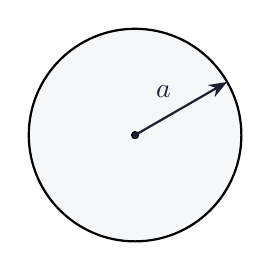
\begin{tikzpicture}[scale=0.9]
  \draw[thick, fill=mygray] (0,0) circle (1.5cm);
  \draw[fill=mydark] (0,0) circle (0.05cm);
  \draw[arrow] (0,0) -- (30:1.5) node[midway, above left] {$a$};
\end{tikzpicture}
\end{minipage}\hfill
\begin{minipage}[c]{0.5\linewidth}
\raggedright
\textbf{Cutoff Frequency Formula:}\\[3pt]
$f_c = \frac{p'_{mn} c}{2\pi a}$ \quad (for TE modes)\\[2pt]
$f_c = \frac{p_{mn} c}{2\pi a}$ \quad (for TM modes)\\[4pt]
Dominant Mode is \textbf{$\text{TE}_{11}$}, where $p'_{11} \approx 1.8412$.
\end{minipage}
\end{tcolorbox}

% ===============================================================================
\section{Stripline and Microstrip Line}
% ===============================================================================

Striplines and microstrip lines are planar transmission lines fabricated on dielectric substrates, forming the core of Microwave Integrated Circuits (MICs).

\begin{tcolorbox}[tikzbox, title={Planar Line Geometries (Stripline vs. Microstrip)}]
\centering
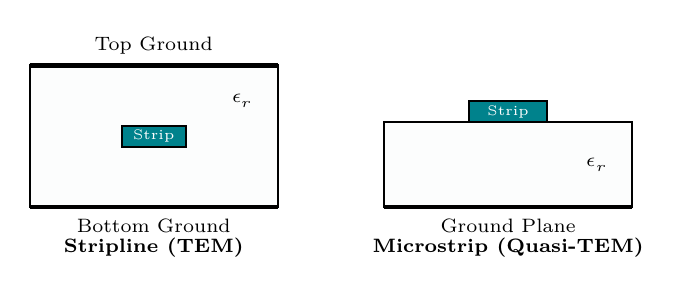
\begin{tikzpicture}[scale=0.9]
  % Stripline
  \draw[thick, fill=mygray!30] (-4,-1) rectangle (-0.5,1);
  \draw[line width=1.5pt] (-4,1) -- (-0.5,1) node[midway, above, font=\scriptsize] {Top Ground};
  \draw[line width=1.5pt] (-4,-1) -- (-0.5,-1) node[midway, below, font=\scriptsize] {Bottom Ground};
  \draw[thick, fill=myteal] (-2.7,-0.15) rectangle (-1.8,0.15) node[midway, font=\tiny\color{white}] {Strip};
  \node[below, font=\scriptsize\bfseries] at (-2.25,-1.3) {Stripline (TEM)};
  
  % Microstrip
  \draw[thick, fill=mygray!30] (1.0,-1.0) rectangle (4.5,0.2);
  \draw[line width=1.5pt] (1.0,-1.0) -- (4.5,-1.0) node[midway, below, font=\scriptsize] {Ground Plane};
  \draw[thick, fill=myteal] (2.2,0.2) rectangle (3.3,0.5) node[midway, font=\tiny\color{white}] {Strip};
  \node[below, font=\scriptsize\bfseries] at (2.75,-1.3) {Microstrip (Quasi-TEM)};
  
  % Labels
  \node[font=\scriptsize] at (-1,0.5) {$\epsilon_r$};
  \node[font=\scriptsize] at (4.0,-0.4) {$\epsilon_r$};
\end{tikzpicture}
\end{tcolorbox}

\subsection{Microstrip Design Formulas}
Because some electric field lines pass through air and others through the substrate, the wave propagation is \textbf{Quasi-TEM}. We define an \textbf{effective dielectric constant} ($\epsilon_{\text{eff}}$):
\begin{equation}
  \epsilon_{\text{eff}} = \frac{\epsilon_r + 1}{2} + \frac{\epsilon_r - 1}{2}\left(1 + 12\frac{h}{w}\right)^{\!-1/2}
\end{equation}
Where $w$ is the strip width and $h$ is substrate thickness. The characteristic impedance is:
\begin{equation}
  Z_0 = \frac{60}{\sqrt{\epsilon_{\text{eff}}}} \ln\left( 8\frac{h}{w} + \frac{w}{4h} \right) \quad \left(\text{for } w/h \le 1\right)
\end{equation}

% ===============================================================================
% MANDATORY QUICK REVISION PAGE
% ===============================================================================
\newpage
\begin{center}
  {\large\bfseries\color{myred} Quick Revision --- Module III}\\[3pt]
  {\small\color{mydark} RF and Microwave Transmission Lines $|$ PE-EC701A}
\end{center}
\noindent{\color{myred}\rule{\linewidth}{1.2pt}}
\vspace{4pt}

\begin{tcolorbox}[formulabox, title={\textbf{Key Formulas at a Glance}}]
\renewcommand{\arraystretch}{1.3}
\begin{tabularx}{\linewidth}{B{4.5cm} X}Coaxial impedance       & $Z_0 = \frac{138}{\sqrt{\epsilon_r}} \log_{10}(b/a)$ \\[4pt]
Rectangular cutoff      & $f_c = \frac{c}{2\sqrt{\epsilon_r}} \sqrt{(m/a)^2 + (n/b)^2}$ \\[4pt]
Guide wavelength        & $\lambda_g = \frac{\lambda_0}{\sqrt{1 - (f_c/f)^2}}$ \\[4pt]
Velocity relation       & $v_p \cdot v_g = c^2$ \quad (in air-filled guide) \\[4pt]
Circular cutoff         & $f_c = \frac{p'_{mn} c}{2\pi a}$ \quad ($\text{TE}_{11}$ dominant, $p'_{11}=1.8412$) \\[4pt]
Effective dielectric    & $\epsilon_{\text{eff}} \approx \frac{\epsilon_r + 1}{2} + \frac{\epsilon_r - 1}{2}(1 + 12h/w)^{-1/2}$
\end{tabularx}
\tcbset{colbacktitle=mygreen, coltitle=white}
\end{tcolorbox}

\begin{tcolorbox}[defbox, title={\textbf{One-Line Definitions}}]
\begin{itemize}[leftmargin=*, itemsep=2.5pt, topsep=0pt]
  \item \textbf{Guide Wavelength:} The axial wavelength of a wave propagating inside a waveguide.
  \item \textbf{Dominant Mode:} The propagation mode with the absolute lowest cutoff frequency.
  \item \textbf{Phase Velocity:} The rate at which the wave's constant-phase wavefronts propagate.
  \item \textbf{Group Velocity:} The speed at which energy and information travel down the line.
  \item \textbf{Quasi-TEM Mode:} A mode resembling TEM but containing small longitudinal fields due to dielectric boundaries.
  \item \textbf{Stripline:} A planar transmission line sandwiched symmetrically between two ground planes.
  \item \textbf{Microstrip:} A planar line on a dielectric substrate with a single bottom ground plane.
\end{itemize}
\end{tcolorbox}

\begin{tcolorbox}[exambox, title={\textbf{Frequently Asked / Viva Questions}}]
\begin{enumerate}[topsep=0pt, label=\textbf{Q\arabic*.}, itemsep=5pt]
  \item \Q{What is the dominant mode in rectangular waveguides and why?}
    The $\text{TE}_{10}$ mode. It has the lowest cutoff frequency ($f_c = c/2a$), meaning it can propagate over the widest single-mode bandwidth.
  \item \Q{Why does a rectangular waveguide act as a high-pass filter?}
    Because it only supports wave propagation above its cutoff frequency ($f > f_c$). Waves below cutoff are attenuated exponentially.
  \item \Q{Explain the relation between phase velocity, group velocity, and the speed of light.}
    In an air-filled guide, $v_p \cdot v_g = c^2$. Since $v_g < c$, the phase velocity $v_p$ must be greater than the speed of light ($v_p > c$).
  \item \Q{What is the dominant mode of a circular waveguide?}
    The $\text{TE}_{11}$ mode, with a cutoff parameter $p'_{11} \approx 1.8412$.
  \item \Q{Why are microstrip lines called Quasi-TEM lines?}
    Because the fields exist in two different mediums (air above, substrate below). The phase velocity mismatch prevents a pure TEM mode.
  \item \Q{How does the characteristic impedance of a coaxial cable depend on conductor sizes?}
    It is proportional to the logarithm of the ratio of the outer radius to inner radius ($Z_0 \propto \ln(b/a)$).
  \item \Q{Why are rectangular waveguides typically designed with $a = 2b$?}
    To maximize the frequency range over which only the dominant $\text{TE}_{10}$ mode propagates before the next mode ($\text{TE}_{20}$ or $\text{TE}_{01}$) turns on.
  \item \Q{What is the physical meaning of the effective dielectric constant ($\epsilon_{\text{eff}}$)?}
    It is the equivalent permittivity of a uniform medium that would produce the same phase velocity as the air-substrate microstrip system.
  \item \Q{What are the advantages of Striplines over Microstrip lines?}
    Striplines are shielded on both sides, which reduces radiation losses and provides better isolation against electromagnetic interference.
  \item \Q{What is the cutoff wavelength ($\lambda_c$) of the dominant mode in a rectangular waveguide?}
    $\lambda_c = 2a$ for the $\text{TE}_{10}$ mode.
  \item \Q{What is a mode chart?}
    A plot of cutoff frequencies for various modes versus waveguide dimensions, used to select optimal waveguide sizes.
  \item \Q{Under what condition does dispersion occur in transmission lines?}
    Dispersion occurs when the phase velocity of the propagating wave depends on frequency ($dv_p/df \ne 0$), causing signals of different frequencies to spread in time.
\end{enumerate}
\tcbset{colbacktitle=mgframe, coltitle=mydark}
\end{tcolorbox}

\begin{tcolorbox}[tikzbox, title={Comparison of Microwave Transmission Lines}]
\renewcommand{\arraystretch}{1.4}
\par\noindent
{\renewcommand{\arraystretch}{1.65}%
\begin{tabularx}{\linewidth}{|B{3.0cm}|Y|Y|Y|}\hline
\textbf{Parameter} & \textbf{Coaxial Line} & \textbf{Rectangular Waveguide} & \textbf{Microstrip Line} \\[4pt]
\hline
\textbf{Mode Supported} & TEM & TE, TM & Quasi-TEM (TE/TM at high f) \\
\hline
\textbf{Cutoff Freq $f_c$} & $0$ (propagates DC) & $f_c = c/2a > 0$ & $0$ (propagates DC) \\[4pt]
\hline
\textbf{Bandwidth} & Very wide & Moderate (between modes) & Very wide \\
\hline
\textbf{Losses} & Moderate & Very low (no dielectric) & High (conductor + radiation) \\
\hline
\textbf{Power Capacity} & Moderate & High & Low \\
\hline
\end{tabularx}
}
\end{tcolorbox}


% -- Module 4 -----------------------------------------------------------------
\modulestart{4}{Equivalent Voltages and Currents for Non-TEM Lines}

\section{Equivalent Voltages and Currents for Non-TEM Lines}
% ===============================================================================

In waveguides supporting TE or TM modes, the physical voltage and current are not uniquely defined because the electric and magnetic fields vary spatially across the guide cross-section. 

\begin{tcolorbox}[defbox]
\textbf{Equivalent Voltage and Current:} Normalized wave quantities defined such that their ratio equals the wave impedance ($Z_w$) and their product represents the power flow ($P$) down the waveguide. They allow waveguides to be analyzed using standard transmission line theory.
\end{tcolorbox}

Let $E_t$ and $H_t$ be the transverse electric and magnetic fields. The equivalent voltage $V(z)$ and current $I(z)$ are defined as:
\begin{align}
  V(z) &= K_V \iint_{S} E_t \cdot e_n \,dS \\
  I(z) &= K_I \iint_{S} H_t \cdot h_n \,dS
\end{align}
Where $e_n, h_n$ are transverse vector mode functions. The normalization is chosen such that:
\begin{equation}
  P = \frac{1}{2} \text{Re}(V I^*) \quad \text{and} \quad \frac{V}{I} = Z_w
\end{equation}

% ===============================================================================
\section{Scattering (S) Parameters}
% ===============================================================================

At high frequencies (microwave range), traditional low-frequency network parameters such as Impedance ($Z$), Admittance ($Y$), and Transmission ($ABCD$) parameters become extremely difficult to measure.

\subsection{Why S-Parameters are Preferred at Microwaves}
\begin{itemize}[leftmargin=*, itemsep=4pt]
  \item \textbf{No Open/Short Circuit Requirements:} Measuring $Z$ and $Y$ parameters requires establishing perfect open and short circuits at the device terminals. At GHz frequencies, lead inductance and stray capacitance make perfect open/shorts impossible to realize.
  \item \textbf{Device Protection:} Creating a short circuit on active microwave devices (like Gunn diodes or high-frequency transistors) can cause them to become unstable and self-oscillate, potentially damaging the device.
  \item \textbf{Matched Terminations:} S-parameters are measured using \textbf{matched loads} (typically $50\,\Omega$). Matched loads are easy to construct at high frequencies and prevent signal reflections.
  \item \textbf{Direct Link to Wave Quantities:} S-parameters relate directly to incident and reflected power waves, which are easily measured using directional couplers.
\end{itemize}

\subsection{S-Parameter Mathematical Definition}
Consider an $N$-port microwave network. At each port $i$, we define normalized incident and reflected wave variables $a_i$ and $b_i$:

\begin{tcolorbox}[tikzbox, title={N-Port Microwave Network Wave Variables}]
\centering
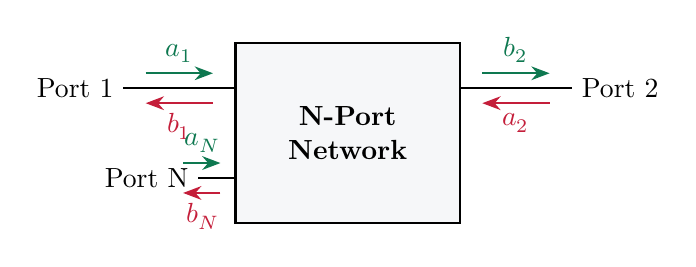
\begin{tikzpicture}[scale=0.95]
  % Central network box
  \draw[thick, fill=mygray] (-1.5,-1.2) rectangle (1.5,1.2);
  \node[font=\bfseries, align=center] at (0,0) {N-Port\\Network};
  
  % Port 1
  \draw[thick] (-3,0.6) -- (-1.5,0.6);
  \node[left] at (-3,0.6) {Port 1};
  \draw[-Stealth, color=mygreen, thick] (-2.7,0.8) -- (-1.8,0.8) node[midway, above] {$a_1$};
  \draw[-Stealth, color=myred, thick] (-1.8,0.4) -- (-2.7,0.4) node[midway, below] {$b_1$};
  
  % Port 2
  \draw[thick] (1.5,0.6) -- (3,0.6);
  \node[right] at (3,0.6) {Port 2};
  \draw[-Stealth, color=mygreen, thick] (1.8,0.8) -- (2.7,0.8) node[midway, above] {$b_2$};
  \draw[-Stealth, color=myred, thick] (2.7,0.4) -- (1.8,0.4) node[midway, below] {$a_2$};
  
  % Port N
  \draw[thick] (-2,-0.6) -- (-1.5,-0.6);
  \node[left] at (-2,-0.6) {Port N};
  \draw[-Stealth, color=mygreen, thick] (-2.2,-0.4) -- (-1.7,-0.4) node[midway, above] {$a_N$};
  \draw[-Stealth, color=myred, thick] (-1.7,-0.8) -- (-2.2,-0.8) node[midway, below] {$b_N$};
\end{tikzpicture}
\end{tcolorbox}

\begin{tcolorbox}[formulabox, title={\textbf{Scattering Parameter Relations}}]
The wave variables $a_i$ (incident) and $b_i$ (reflected) are related to port voltages $V_i$, currents $I_i$, and characteristic impedance $Z_0$ by:
\begin{align}
  a_i &= \frac{V_i + I_i Z_0}{2\sqrt{Z_0}} \quad (\text{incident wave}) \\
  b_i &= \frac{V_i - I_i Z_0}{2\sqrt{Z_0}} \quad (\text{reflected wave})
\end{align}
The linear relationship between the waves is expressed in matrix form as:
\begin{equation}
  [b] = [S][a]
\end{equation}
For a 2-port network:
\begin{equation}
  \begin{bmatrix} b_1 \\ b_2 \end{bmatrix} = \begin{bmatrix} S_{11} & S_{12} \\ S_{21} & S_{22} \end{bmatrix} \begin{bmatrix} a_1 \\ a_2 \end{bmatrix}
\end{equation}
Where:
\begin{itemize}[leftmargin=1.5em, itemsep=1.5pt]
  \item[] $S_{ii} = \left. \frac{b_i}{a_i} \right|_{a_k=0 \text{ for } k \ne i}$ is the reflection coefficient at port $i$ when all other ports are matched.
  \item[] $S_{ij} = \left. \frac{b_i}{a_j} \right|_{a_k=0 \text{ for } k \ne j}$ is the transmission coefficient from port $j$ to port $i$ under matched termination.
\end{itemize}
\end{tcolorbox}

% ===============================================================================
\section{Properties of the S-Matrix}
% ===============================================================================

The S-matrix possesses key mathematical properties governed by reciprocity and conservation of energy.

\subsection{Symmetric Property for Reciprocal Networks}
A network is reciprocal if the transmission of energy from port $i$ to port $j$ is identical to transmission from $j$ to $i$.
\begin{tcolorbox}[defbox]
\textbf{Symmetric Property:} The scattering matrix of a reciprocal network is symmetric.
\begin{equation}
  [S]^T = [S] \quad \implies \quad S_{ij} = S_{ji}
\end{equation}
\end{tcolorbox}

\subsubsection{Derivation of the Reciprocal Property}
For a reciprocal network, the impedance matrix $[Z]$ is symmetric:
\begin{equation*}
  [Z]^T = [Z]
\end{equation*}
The relationship between S-parameters and Z-parameters (normalized to $Z_0 = 1$) is:
\begin{equation}
  [S] = ([Z] - [I])([Z] + [I])^{-1}
\end{equation}
Taking the transpose of both sides:
\begin{align*}
  [S]^T &= \left[ ([Z] - [I])([Z] + [I])^{-1} \right]^T \\
  &= \left( ([Z] + [I])^{-1} \right)^T \cdot ([Z] - [I])^T \\
  &= \left( ([Z] + [I])^T \right)^{-1} \cdot ([Z]^T - [I]^T)
\end{align*}
Since $[Z]^T = [Z]$ and the identity matrix is symmetric ($[I]^T = [I]$):
\begin{equation*}
  [S]^T = ([Z] + [I])^{-1} ([Z] - [I])
\end{equation*}
Since matrices of the form $([Z] \pm [I])$ commute:
\begin{equation*}
  ([Z] + [I])^{-1} ([Z] - [I]) = ([Z] - [I]) ([Z] + [I])^{-1} = [S]
\end{equation*}
Thus, we prove:
\begin{equation}
  [S]^T = [S] \quad \text{(Q.E.D.)}
\end{equation}

\subsection{Unitary Property for Lossless Networks}
In a lossless network, no real power is dissipated; the total power entering the network must equal the total power leaving it.
\begin{tcolorbox}[defbox]
\textbf{Unitary Property:} The S-matrix of a lossless network is unitary.
\begin{equation}
  [S]^{*, T} [S] = [I] \quad \text{or} \quad [S]^\dagger [S] = [I]
\end{equation}
\end{tcolorbox}

\subsubsection{Derivation of the Lossless Property}
The total power entering an $N$-port network is the sum of incident powers:
\begin{equation*}
  P_{in} = \frac{1}{2} \sum_{i=1}^N |a_i|^2 = \frac{1}{2} [a]^{*, T} [a]
\end{equation*}
The total power leaving the network is the sum of reflected powers:
\begin{equation*}
  P_{out} = \frac{1}{2} \sum_{i=1}^N |b_i|^2 = \frac{1}{2} [b]^{*, T} [b]
\end{equation*}
Since the network is lossless, conservation of energy dictates $P_{in} = P_{out}$:
\begin{equation*}
  [a]^{*, T} [a] = [b]^{*, T} [b]
\end{equation*}
Substituting $[b] = [S][a]$ and taking its conjugate transpose $[b]^{*, T} = [a]^{*, T} [S]^{*, T}$:
\begin{equation*}
  [a]^{*, T} [a] = [a]^{*, T} [S]^{*, T} [S] [a]
\end{equation*}
This equation must hold for any arbitrary incident wave vector $[a]$. Hence:
\begin{equation}
  [S]^{*, T} [S] = [I] \quad \text{(Q.E.D.)}
\end{equation}

% ===============================================================================
% MANDATORY QUICK REVISION PAGE
% ===============================================================================
\newpage
\begin{center}
  {\large\bfseries\color{myred} Quick Revision --- Module IV}\\[3pt]
  {\small\color{mydark} Microwave Network Analysis $|$ PE-EC701A}
\end{center}
\noindent{\color{myred}\rule{\linewidth}{1.2pt}}
\vspace{4pt}

\begin{tcolorbox}[formulabox, title={\textbf{Key Formulas at a Glance}}]
\renewcommand{\arraystretch}{1.3}
\begin{tabularx}{\linewidth}{B{4.5cm} X}Incident wave variable  & $a_i = \frac{V_i + I_i Z_0}{2\sqrt{Z_0}}$ \\[4pt]
Reflected wave variable  & $b_i = \frac{V_i - I_i Z_0}{2\sqrt{Z_0}}$ \\[4pt]
Reciprocal condition    & $[S]^T = [S] \quad \implies S_{ij} = S_{ji}$ \\[4pt]
Lossless condition      & $[S]^{*, T} [S] = [I] \quad \implies \sum_{k=1}^N S_{ki}^* S_{kj} = \delta_{ij}$ \\[4pt]
Reflection \& VSWR      & $S_{11} = \Gamma = \frac{\text{VSWR}-1}{\text{VSWR}+1}$
\end{tabularx}
\tcbset{colbacktitle=mygreen, coltitle=white}
\end{tcolorbox}

\begin{tcolorbox}[defbox, title={\textbf{One-Line Definitions}}]
\begin{itemize}[leftmargin=*, itemsep=2.5pt, topsep=0pt]
  \item \textbf{S-Parameters:} Network parameters relating incident and reflected voltage waves.
  \item \textbf{Reciprocal Network:} A passive network where transmission coefficients are independent of propagation direction.
  \item \textbf{Lossless Network:} A network that conserves RF power, having zero internal power dissipation.
  \item \textbf{Unitary Matrix:} A complex matrix whose conjugate transpose is also its inverse.
  \item \textbf{Insertion Loss:} The attenuation of a signal passing through a network, given by $-20 \log_{10}|S_{ji}|$ dB.
  \item \textbf{Return Loss:} A measure of reflection mismatch at a port, given by $-20 \log_{10}|S_{ii}|$ dB.
  \item \textbf{Matched Termination:} Connecting a load equal to the characteristic impedance, preventing reflection.
\end{itemize}
\end{tcolorbox}

\begin{tcolorbox}[exambox, title={\textbf{Frequently Asked / Viva Questions}}]
\begin{enumerate}[topsep=0pt, label=\textbf{Q\arabic*.}, itemsep=5pt]
  \item \Q{Why are Z and Y parameters not suitable for microwave frequencies?}
    Because they require open and short circuit terminations. At microwave frequencies, parasitics make open/shorts impossible, and shorts can damage active devices.
  \item \Q{What is the physical meaning of $S_{11}$ and $S_{21}$?}
    $S_{11}$ is the input reflection coefficient when port 2 is matched. $S_{21}$ is the forward transmission coefficient from port 1 to port 2 when port 2 is matched.
  \item \Q{State the unitary property of the S-matrix in summation form.}
    For a lossless network, $\sum_{k=1}^N |S_{ki}|^2 = 1$ (unity relation) and $\sum_{k=1}^N S_{ki}^* S_{kj} = 0$ for $i \ne j$ (zero relation).
  \item \Q{Prove that a 1-port network with a matched load has $S_{11} = 0$.}
    A matched load absorbs all incident energy, generating zero reflected wave ($b_1 = 0$), so $S_{11} = b_1/a_1 = 0$.
  \item \Q{What is the relationship between S-parameters and ABCD parameters?}
    ABCD parameters relate input voltage and current to output voltage and current. They are cascading parameters, unlike S-parameters which relate incident/reflected waves.
  \item \Q{Why are S-parameters measured relative to a specific reference impedance (usually $50\,\Omega$)?}
    Because wave variables $a$ and $b$ are normalized to $\sqrt{Z_0}$. Changing $Z_0$ changes the values of the S-parameters.
  \item \Q{What does a return loss of $\infty$ dB represent?}
    It represents a perfect match ($S_{11} = 0$), where no signal is reflected back.
  \item \Q{How do you check if an S-matrix represents a physical, passive network?}
    The magnitude of all elements must be less than or equal to one ($|S_{ij}| \le 1$), and the network must not generate net power (the eigenvalues of $[S]^{*,T}[S]$ must be $\le 1$).
  \item \Q{What is the relation between S-parameters and VSWR?}
    $\text{VSWR} = \frac{1 + |S_{ii}|}{1 - |S_{ii}|}$.
  \item \Q{Under what conditions is the ABCD matrix preferred over the S-matrix?}
    When cascading multiple microwave networks in series, because the overall ABCD matrix is simply the product of individual ABCD matrices ($[ABCD]_{\text{total}} = [A] \cdot [B] \dots$).
  \item \Q{What is equivocation in the context of network transmission?}
    It is the power lost or diverted due to reflection and mismatch at network junctions.
  \item \Q{Why is the S-matrix symmetric for reciprocal networks?}
    Because the underlying electromagnetic materials are isotropic, yielding symmetric impedance ($[Z]$) and admittance ($[Y]$) matrices, which mathematically maps to $[S]^T = [S]$.
\end{enumerate}
\tcbset{colbacktitle=mgframe, coltitle=mydark}
\end{tcolorbox}

\begin{tcolorbox}[tikzbox, title={Comparison of Z, Y, ABCD, and S-Parameters}]
\renewcommand{\arraystretch}{1.4}
\par\noindent
{\renewcommand{\arraystretch}{1.65}%
\begin{tabularx}{\linewidth}{|B{2.8cm}|Y|Y|Y|}\hline
\textbf{Parameters} & \textbf{Independent Variables} & \textbf{Dependent Variables} & \textbf{Terminations Required} \\[4pt]
\hline
\textbf{Z Parameters} & Currents ($I_1, I_2$) & Voltages ($V_1, V_2$) & Open Circuit ($I = 0$) \\[4pt]
\hline
\textbf{Y Parameters} & Voltages ($V_1, V_2$) & Currents ($I_1, I_2$) & Short Circuit ($V = 0$) \\[4pt]
\hline
\textbf{ABCD Params} & Output variables ($V_2, -I_2$) & Input variables ($V_1, I_1$) & Open / Short depending on parameter \\[4pt]
\hline
\textbf{S Parameters} & Incident Waves ($a_1, a_2$) & Reflected Waves ($b_1, b_2$) & Matched Termination ($a = 0$) \\[4pt]
\hline
\end{tabularx}
}
\end{tcolorbox}


% -- Module 5 -----------------------------------------------------------------
\modulestart{5}{Microwave Passive Components}

\section{Microwave Passive Components}
% ===============================================================================

Microwave passive components route, split, attenuate, or filter RF signals without adding energy to the system.

\subsection{Directional Coupler}
A directional coupler is a 4-port device that couples a specific fraction of power from one transmission line to another in a directive manner.
\begin{itemize}[leftmargin=*, itemsep=3pt]
  \item \textbf{Port 1 (Input), Port 2 (Through), Port 3 (Coupled), Port 4 (Isolated).}
  \item \textbf{Key Parameters:} Coupling ($C$), Directivity ($D$), and Isolation ($I$).
\end{itemize}

\begin{tcolorbox}[formulabox, title={\textbf{Directional Coupler Metrics \& S-Matrix}}]
\begin{align}
  \text{Coupling Factor } C &= -20 \log_{10} \left| \frac{P_3}{P_1} \right| \quad (\text{dB}) \\
  \text{Directivity } D &= -20 \log_{10} \left| \frac{P_4}{P_3} \right| \quad (\text{dB}) \\
  \text{Isolation } I &= -20 \log_{10} \left| \frac{P_4}{P_1} \right| = C + D \quad (\text{dB})
\end{align}
The S-matrix of an ideal symmetric reciprocal coupler (normalized to matched ports) is:
\begin{equation}
  [S] = \begin{bmatrix} 0 & p & j q & 0 \\ p & 0 & 0 & j q \\ j q & 0 & 0 & p \\ 0 & j q & p & 0 \end{bmatrix} \quad (\text{with } p^2 + q^2 = 1)
\end{equation}
\end{tcolorbox}

\subsection{Magic Tee (Hybrid Tee)}
A Magic Tee is a 4-port waveguide junction combining an E-plane (series) arm and an H-plane (shunt) arm. It is used as a mixer or duplexer.

\begin{tcolorbox}[tikzbox, title={Magic Tee Port Configuration Scheme}]
\begin{minipage}[c]{0.45\linewidth}
\centering
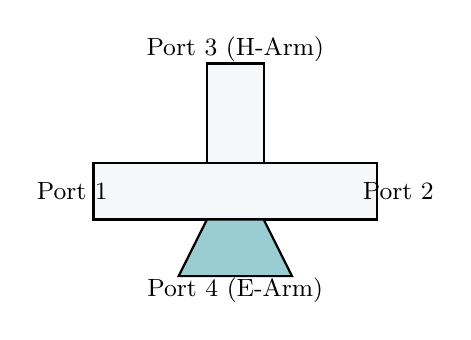
\begin{tikzpicture}[scale=0.9, every node/.style={font=\small}]
  % Drawing Magic Tee schematic representation
  \draw[thick, fill=mygray] (-2,-0.4) rectangle (2,0.4);
  \draw[thick, fill=mygray] (-0.4,0.4) rectangle (0.4,1.8); % H-plane arm
  \draw[thick, fill=myteal!40] (-0.4,-0.4) -- (-0.8,-1.2) -- (0.8,-1.2) -- (0.4,-0.4) -- cycle; % E-plane arm (projected down)
  
  \node at (-2.3,0) {Port 1};
  \node at (2.3,0) {Port 2};
  \node at (0,2.0) {Port 3 (H-Arm)};
  \node at (0,-1.4) {Port 4 (E-Arm)};
\end{tikzpicture}
\end{minipage}\hfill
\begin{minipage}[c]{0.5\linewidth}
\raggedright
\textbf{Operation:}\\[3pt]
$\bullet$ Feed Port 3 $\to$ Outputs 1 \& 2 in-phase ($V_1 = V_2$)\\[2pt]
$\bullet$ Feed Port 4 $\to$ Outputs 1 \& 2 out-of-phase ($V_1 = -V_2$)\\[2pt]
$\bullet$ Feed Port 1 \& 2 $\to$ Sum at Port 3, Diff at Port 4
\end{minipage}
\end{tcolorbox}

\begin{tcolorbox}[formulabox, title={\textbf{Magic Tee S-Matrix}}]
For matched and isolated E and H ports:
\begin{equation}
  [S] = \frac{1}{\sqrt{2}} \begin{bmatrix} 0 & 0 & 1 & 1 \\ 0 & 0 & 1 & -1 \\ 1 & 1 & 0 & 0 \\ 1 & -1 & 0 & 0 \end{bmatrix}
\end{equation}
\end{tcolorbox}

\subsection{Waveguide Attenuators}
Microwave attenuators are passive components used to reduce the amplitude or power level of a signal by a desired amount (expressed in dB) while maintaining impedance matching.
\begin{itemize}[leftmargin=*, itemsep=3pt]
  \item \textbf{Fixed Attenuator:} Employs a thin resistive card placed at the center of the waveguide parallel to the maximum electric field ($TE_{10}$ mode). It absorbs RF energy and dissipates it as heat.
  \item \textbf{Rotary Vane Variable Attenuator:} Consists of three sections: a center circular waveguide containing a rotatable resistive card, positioned between two rectangular-to-circular transitions with fixed horizontal cards.
  \begin{itemize}[leftmargin=*, itemsep=2.5pt, topsep=0pt]
    \item When the center card is rotated by an angle $\theta$ relative to the incoming E-field, the parallel component is absorbed. The perpendicular component ($E \cos\theta$) passes.
    \item Passing through the output transition (which is horizontal), the field is further reduced by $\cos\theta$, resulting in an output amplitude of $E_0 = E \cos^2\theta$.
    \item \textbf{Attenuation Equation:}
      \begin{equation}
        A_{\text{dB}} = -20 \log_{10}(\cos^2\theta) = -40 \log_{10}(\cos\theta)
      \end{equation}
      This attenuation depends strictly on rotation angle $\theta$, making it highly precise and frequency-independent.
  \end{itemize}
\end{itemize}

\subsection{Power Divider (T-Junction and Wilkinson)}
Power dividers are passive 3-port networks used to split an input signal into two or more output signals of lesser power.
\begin{itemize}[leftmargin=*, itemsep=3pt]
  \item \textbf{Reciprocal Lossless 3-Port Limitation:} By S-matrix properties, it is mathematically impossible for a 3-port junction to be simultaneously reciprocal, lossless, and matched at all ports.
  \item \textbf{T-Junction Power Divider:} A simple lossless reciprocal 3-port divider (E-plane or H-plane waveguide junction or microstrip line). Since it is lossless and reciprocal, it cannot be matched at all ports simultaneously (typically the output ports are mismatched, leading to reflections).
  \item \textbf{Wilkinson Power Divider:} A reciprocal 3-port network that achieves matching at all ports simultaneously and provides high isolation between the output ports by utilizing internal loss under mismatch. It is lossless when the output ports are matched and balanced.
\end{itemize}

\begin{tcolorbox}[tikzbox, title={Wilkinson Power Divider Transmission Line Layout}]
\centering
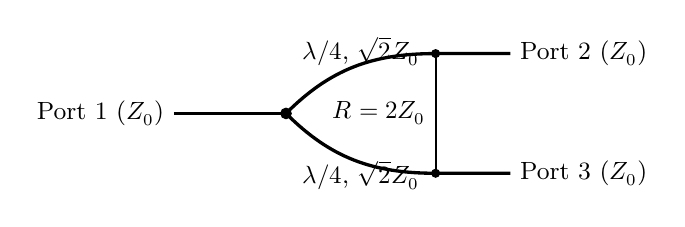
\begin{tikzpicture}[scale=0.95, every node/.style={font=\small}]
  % Input line
  \draw[very thick] (0,0) -- (1.5,0);
  \node[left] at (0,0) {Port 1 ($Z_0$)};
  
  % Split junction
  \filldraw (1.5,0) circle (2pt);
  
  % Upper branch (quarter-wave transformer)
  \draw[very thick] (1.5,0) to[out=45, in=180] (3.5,0.8) -- (4.5,0.8);
  \node[above] at (2.5,0.5) {$\lambda/4$, $\sqrt{2}Z_0$};
  \node[right] at (4.5,0.8) {Port 2 ($Z_0$)};
  
  % Lower branch (quarter-wave transformer)
  \draw[very thick] (1.5,0) to[out=-45, in=180] (3.5,-0.8) -- (4.5,-0.8);
  \node[below] at (2.5,-0.5) {$\lambda/4$, $\sqrt{2}Z_0$};
  \node[right] at (4.5,-0.8) {Port 3 ($Z_0$)};
  
  % Isolation Resistor
  \draw[thick] (3.5,0.8) -- (3.5,-0.8);
  \filldraw (3.5,0.8) circle (1.5pt);
  \filldraw (3.5,-0.8) circle (1.5pt);
  \node[left] at (3.5,0) {$R = 2Z_0$};
\end{tikzpicture}
\end{tcolorbox}

\begin{tcolorbox}[formulabox, title={\textbf{Wilkinson Power Divider S-Matrix}}]
For design parameters with quarter-wave line impedance of $Z_0\sqrt{2}$ and an isolation resistor of $2Z_0$, the S-matrix of an ideal symmetric Wilkinson power divider matched at all three ports is:
\begin{equation}
  [S] = -\frac{j}{\sqrt{2}} \begin{bmatrix} 0 & 1 & 1 \\ 1 & 0 & 0 \\ 1 & 0 & 0 \end{bmatrix}
\end{equation}
When ports 2 and 3 are matched, no current flows through the isolation resistor $2Z_0$, and the power is split equally with zero loss ($S_{21} = S_{31} = -3\text{ dB}$).
\end{tcolorbox}

\subsection{Cavity Resonators}
A microwave cavity resonator is a metallic enclosure that confines electromagnetic energy inside a cavity, storing it in standing waves.
\begin{itemize}[leftmargin=*, itemsep=3pt]
  \item \textbf{Mechanism:} Unlike lumped LC circuits which suffer from high radiation and conductor losses at gigahertz frequencies, cavity resonators completely enclose fields to achieve extremely high Q-factors ($10^3$ to $10^5$).
  \item \textbf{Rectangular Cavity Resonator:} Formed by closing both ends of a rectangular waveguide of dimensions $a \times b$ at a distance $d$ (along the z-axis). Resonance occurs when the guide length $d$ is an integer multiple of half-guide-wavelengths ($d = p \lambda_g / 2$).
\end{itemize}

\begin{tcolorbox}[formulabox, title={\textbf{Cavity Resonance \& Quality Factor}}]
The resonant frequency $f_{mnp}$ for $\text{TE}_{mnp}$ or $\text{TM}_{mnp}$ modes in a rectangular cavity filled with dielectric ($\epsilon_r$) is:
\begin{equation}
  f_{mnp} = \frac{c}{2\sqrt{\epsilon_r}} \sqrt{\left(\frac{m}{a}\right)^{\!2} + \left(\frac{n}{b}\right)^{\!2} + \left(\frac{p}{d}\right)^{\!2}} \quad (\text{Hz})
\end{equation}
The \textbf{Quality Factor ($Q$)} measures the energy storage efficiency of the resonator:
\begin{equation}
  Q = 2\pi \frac{\text{Energy Stored}}{\text{Energy Dissipated per cycle}} = \omega \frac{W}{P_L}
\end{equation}
\begin{itemize}[leftmargin=1.5em, itemsep=2pt, topsep=2pt]
  \item \textbf{Unloaded $Q$ ($Q_0$):} Internal $Q$ of the cavity itself, accounting for conductor wall losses ($Q_c$) and dielectric losses ($Q_d$): $1/Q_0 = 1/Q_c + 1/Q_d$.
  \item \textbf{Loaded $Q$ ($Q_L$):} Accounts for both internal cavity losses and external circuit load losses ($Q_e$):
    \begin{equation}
      \frac{1}{Q_L} = \frac{1}{Q_0} + \frac{1}{Q_e}
    \end{equation}
\end{itemize}
\end{tcolorbox}

% ===============================================================================
\section{Microwave Semiconductor Devices}
% ===============================================================================

\subsection{Gunn Diode}
The Gunn diode is not a junction diode but a bulk semiconductor device (typically GaAs) that exhibits negative differential resistance due to the \textbf{transferred-electron mechanism (RWH Theory)}.
\begin{itemize}[leftmargin=*, itemsep=3pt]
  \item Under high electric fields, electrons transfer from a high-mobility lower valley to a low-mobility upper valley in the conduction band, causing current to drop as voltage increases.
\end{itemize}

\subsection{IMPATT Diode}
The \textbf{IMPATT (IMPact ionization Avalanche Transit Time)} diode operates under reverse breakdown, utilizing avalanche multiplication and carrier transit time delays to generate a $180^\circ$ phase shift (negative resistance) at microwave frequencies.

\subsection{PIN Diode}
Constructed with a high-resistivity intrinsic semiconductor sandwiched between p-type and n-type regions.
\begin{itemize}[leftmargin=*, itemsep=3pt]
  \item \textbf{Under Forward Bias:} Behaves as a low-resistance resistor ($\sim 1\,\Omega$), passing RF.
  \item \textbf{Under Reverse Bias:} Behaves as a high resistance in parallel with a small capacitance, blocking RF. Ideal as a high-speed RF switch.
\end{itemize}

\subsection{Schottky Barrier Diode}
The Schottky barrier diode consists of a metal-semiconductor rectifying junction (e.g., gold or tungsten on n-type GaAs).
\begin{itemize}[leftmargin=*, itemsep=3pt]
  \item \textbf{Working:} Unlike standard p-n diodes, it is a \textbf{majority carrier device}. When forward-biased, electrons from the semiconductor are injected into the metal (thermionic emission) where they rapidly lose energy.
  \item \textbf{High-Frequency Advantage:} Since there is \textbf{zero minority carrier storage time} (no charge storage delay), the diode can switch states in picoseconds, making it ideal for low-noise mixers, detectors, and switching circuits up to THz frequencies.
\end{itemize}

\subsection{GaAs MESFET}
The Metal-Semiconductor Field Effect Transistor (MESFET) replaces the traditional insulated gate of a MOSFET with a metal Schottky barrier gate deposited directly on an n-type GaAs channel.
\begin{itemize}[leftmargin=*, itemsep=3pt]
  \item \textbf{Operation:} Gate voltage modulates the depletion region width beneath the Schottky gate, controlling channel conduction.
  \item \textbf{Key Feature:} The high electron mobility of GaAs (compared to Silicon) yields extremely high electron drift velocities, enabling high cut-off frequencies ($f_T > 100\,\text{GHz}$).
\end{itemize}

\subsection{HEMT (High Electron Mobility Transistor)}
The HEMT (or MODFET) is a heterostructure field-effect transistor that utilizes the junction between materials of different bandgaps (e.g., AlGaAs and GaAs).
\begin{itemize}[leftmargin=*, itemsep=3pt]
  \item \textbf{2DEG formation:} Free electrons from the n-doped AlGaAs layer migrate across the heterojunction to the undoped GaAs side, where they are trapped in a quantum well, forming a thin sheet of charge called a \textbf{Two-Dimensional Electron Gas (2DEG)}.
  \item \textbf{Carrier Mobility:} Because the 2DEG channel lies in an undoped GaAs layer, the moving electrons experience \textbf{no ionized impurity scattering}. This results in extremely high carrier mobilities and noise figures near zero, making HEMTs the industry standard for Low Noise Amplifiers (LNAs).
\end{itemize}

% ===============================================================================
\section{Microwave Tubes (Linear-Beam and Cross-Field)}
% ===============================================================================

Traditional vacuum tubes fail at microwave frequencies due to \textbf{transit-time effects} (the time taken by electrons to cross the grid becomes comparable to the RF cycle period, causing grid loading). Microwave tubes overcome this by utilizing electron velocity modulation.

\subsection{Klystron (Two-Cavity and Reflex)}
In a Two-Cavity Klystron, an electron beam passes through a \textbf{buncher cavity} where a small RF signal velocity-modulates the electrons (speeding up some, slowing down others). During travel through the drift space, they form \textbf{bunches} that yield strong RF currents in the \textbf{catcher cavity}.

\begin{tcolorbox}[tikzbox, title={Applegate Diagram of Velocity Modulation}]
\centering
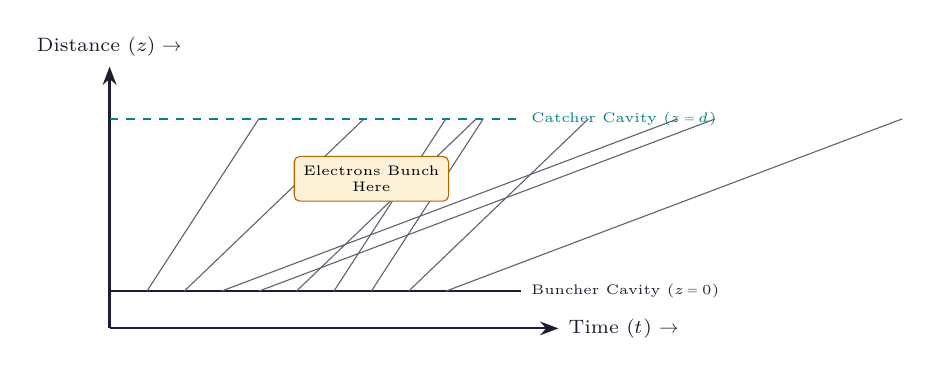
\begin{tikzpicture}[scale=0.95]
  \draw[arrow] (0,0) -- (6,0) node[right, font=\scriptsize] {Time ($t$) $\to$};
  \draw[arrow] (0,0) -- (0,3.5) node[above, font=\scriptsize] {Distance ($z$) $\to$};
  
  % Buncher position
  \draw[line] (0,0.5) -- (5.5,0.5) node[right, font=\tiny\color{myred}] {Buncher Cavity ($z=0$)};
  \draw[line, dashed, color=myteal] (0,2.8) -- (5.5,2.8) node[right, font=\tiny\color{myteal}] {Catcher Cavity ($z=d$)};
  
  % Electron paths (slopes represent velocities)
  \foreach \t in {0.5, 1.0, 1.5, 2.0, 2.5, 3.0, 3.5, 4.0, 4.5} {
    % Modulate slope based on sin function of start time
    \pgfmathsetmacro{\slope}{0.5 + 0.35*sin((\t-2.5)*180/1.5)}
    \draw[color=mydark!70, thin] (\t, 0.5) -- (\t + 1.2/\slope, 2.8);
  }
  
  \node[draw=myamber, fill=hdramber, rounded corners=2pt, font=\tiny, align=center] at (3.5,2.0) {Electrons Bunch\\Here};
\end{tikzpicture}
\end{tcolorbox}

\textbf{Reflex Klystron:} Uses a single cavity and a \textbf{repeller electrode} to return electrons back through the cavity, creating feedback and oscillation.

\subsection{Traveling Wave Tube (TWT)}
A TWT is a non-resonant linear amplifier. It utilizes a \textbf{slow-wave structure} (usually a wire helix) to slow down the RF wave phase velocity so it matches the electron beam velocity, allowing continuous energy transfer along the entire tube length.

\begin{tcolorbox}[tikzbox, title={Traveling Wave Tube (TWT) Concept}]
\centering
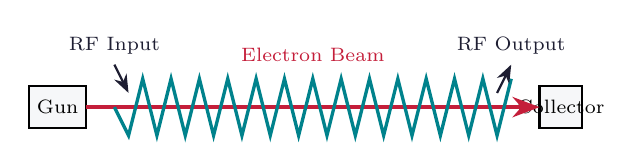
\begin{tikzpicture}[scale=0.9, every node/.style={font=\scriptsize}]
  % Electron Gun
  \draw[thick, fill=mygray] (0,0.4) rectangle (0.8,1.0) node[midway] {Gun};
  % Collector
  \draw[thick, fill=mygray] (7.2,0.4) rectangle (7.8,1.0) node[midway] {Collector};
  
  % Electron Beam
  \draw[line width=1.5pt, color=myred, -Stealth] (0.8,0.7) -- (7.2,0.7);
  \node[above, color=myred, font=\scriptsize] at (4,1.2) {Electron Beam};
  
  % Helix line (slow wave structure)
  \draw[very thick, color=myteal] (1.2,0.7) 
    \foreach \x in {1.4,1.8,2.2,2.6,3.0,3.4,3.8,4.2,4.6,5.0,5.4,5.8,6.2,6.6} {
      -- (\x, 0.3) -- (\x+0.2, 1.1)
    };
    
  \draw[arrow] (1.2,1.3) node[above] {RF Input} -- (1.4,0.9);
  \draw[arrow] (6.6,0.9) -- (6.8,1.3) node[above] {RF Output};
\end{tikzpicture}
\end{tcolorbox}

\subsection{Magnetron}
A cavity magnetron is a high-power cross-field (M-type) microwave oscillator.
\begin{itemize}[leftmargin=*, itemsep=3pt]
  \item \textbf{Crossed Fields:} Direct electric field ($\vec{E}$) between anode and cathode, and axial magnetic field ($\vec{B}$) perpendicular to the electric field.
  \item \textbf{Working:} Electrons from the cathode spiral in the crossed fields, interacting with the resonant cavities in the anode block. In the \textbf{$\pi$-mode}, adjacent cavities oscillate $180^\circ$ out-of-phase, forcing electrons into spokes that continuously feed energy to the cavities.
\end{itemize}

\begin{tcolorbox}[tikzbox, title={Cavity Magnetron Cross-Section}]
\begin{minipage}[c]{0.45\linewidth}
\centering
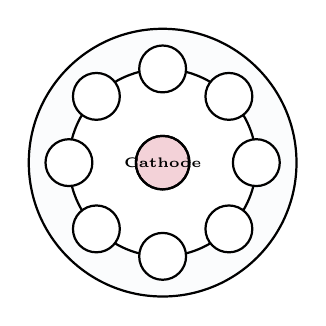
\begin{tikzpicture}[scale=0.85]
  % Outer anode ring
  \draw[thick, fill=mygray!40] (0,0) circle (2.0cm);
  \draw[thick, fill=white] (0,0) circle (1.4cm);
  
  % Inner cathode
  \draw[thick, fill=myred!20] (0,0) circle (0.4cm);
  \node[font=\tiny\bfseries] at (0,0) {Cathode};
  
  % 8 Cavities
  \foreach \angle in {0, 45, 90, 135, 180, 225, 270, 315} {
    \draw[thick, fill=white] (\angle:1.4) circle (0.35cm);
  }
  
  % Re-draw cathode outline
  \draw[thick] (0,0) circle (0.4cm);
\end{tikzpicture}
\end{minipage}\hfill
\begin{minipage}[c]{0.5\linewidth}
\raggedright
$\bullet$ \textbf{Anode Block:} 8 Cavities\\[3pt]
$\bullet$ \textbf{Crossed Fields:} $\vec{E}$ radial, $\vec{B}$ perpendicular to page ($\odot$)\\[3pt]
$\bullet$ Electrons form rotating "spokes"
\end{minipage}
\end{tcolorbox}

% ===============================================================================
% MANDATORY QUICK REVISION PAGE
% ===============================================================================
\newpage
\begin{center}
  {\large\bfseries\color{myred} Quick Revision --- Module V}\\[3pt]
  {\small\color{mydark} Passive and Active Microwave Devices $|$ PE-EC701A}
\end{center}
\noindent{\color{myred}\rule{\linewidth}{1.2pt}}
\vspace{4pt}

\begin{tcolorbox}[formulabox, title={\textbf{Key Formulas at a Glance}}]
\renewcommand{\arraystretch}{1.3}
\begin{tabularx}{\linewidth}{B{4.5cm} X}Coupling Factor ($C$)   & $C = -20 \log_{10} |S_{31}| = -20 \log_{10} |P_3/P_1|^{1/2}$ \\[4pt]
Directivity ($D$)       & $D = -20 \log_{10} |S_{43}| = -20 \log_{10} |P_4/P_3|^{1/2}$ \\[4pt]
Isolation ($I$)         & $I = C + D = -20 \log_{10} |S_{41}|$ \\[4pt]
Wilkinson S-matrix      & $[S] = -\frac{j}{\sqrt{2}} \begin{bmatrix} 0 & 1 & 1 \\ 1 & 0 & 0 \\ 1 & 0 & 0 \end{bmatrix}$ \\[4pt]
Resonator frequency     & $f_0 = \frac{c}{2\sqrt{\epsilon_r}} \sqrt{(m/a)^2 + (n/b)^2 + (p/d)^2}$ \\[4pt]
Rotary Vane Attenuation & $A_{\text{dB}} = -40 \log_{10}(\cos\theta)$
\end{tabularx}
\tcbset{colbacktitle=mygreen, coltitle=white}
\end{tcolorbox}

\begin{tcolorbox}[defbox, title={\textbf{One-Line Definitions}}]
\begin{itemize}[leftmargin=*, itemsep=2.5pt, topsep=0pt]
  \item \textbf{Magic Tee:} A 4-port waveguide hybrid junction combining E and H arms to perform sum and difference processing.
  \item \textbf{Gunn Effect:} The emission of coherent microwave oscillations from bulk semiconductor material under high fields.
  \item \textbf{Negative Resistance:} A device property where current decreases with increasing voltage, enabling amplification.
  \item \textbf{Transit Time:} The time taken by a charge carrier to traverse the active length of a device.
  \item \textbf{Slow-Wave Structure:} A wire helix or waveguide circuit that reduces RF phase velocity to match electron beam speed.
  \item \textbf{Bunching:} The process in microwave tubes where velocity-modulated electrons form spatial charge clusters.
  \item \textbf{Applegate Diagram:} A distance-time graphical plot showing electron bunching trajectories in klystrons.
  \item \textbf{Schottky Diode:} A metal-semiconductor junction diode relying on majority carriers for zero reverse recovery delay.
  \item \textbf{GaAs MESFET:} Field-effect transistor using a Schottky barrier metal gate directly on a GaAs channel.
  \item \textbf{HEMT:} High Electron Mobility Transistor; uses a heterojunction to form a high-speed, low-noise 2DEG layer.
  \item \textbf{Rotary Vane Attenuator:} A frequency-independent waveguide attenuator calibrated via a rotating resistive vane.
\end{itemize}
\end{tcolorbox}

\begin{tcolorbox}[exambox, title={\textbf{Frequently Asked / Viva Questions}}]
\begin{enumerate}[topsep=0pt, label=\textbf{Q\arabic*.}, itemsep=5pt]
  \item \Q{State the matching and isolation properties of a Magic Tee.}
    If ports 3 (H-port) and 4 (E-port) are matched, they are isolated from each other ($S_{34} = S_{43} = 0$). Additionally, collinear ports 1 and 2 are isolated from each other ($S_{12} = S_{21} = 0$).
  \item \Q{Why are conventional triodes and pentodes useless at microwave frequencies?}
    Due to transit-time effects and lead inductance/capacitance, which cause severe grid loading and phase shifts that prevent amplification.
  \item \Q{Explain the basic principle of velocity modulation in a Klystron.}
    The input RF voltage in the buncher cavity accelerates electrons during the positive half-cycle and decelerates them during the negative half-cycle, converting a uniform velocity beam into a velocity-modulated beam.
  \item \Q{How does a TWT differ from a Klystron?}
    A Klystron uses resonant cavities for narrow-band interaction, while a TWT uses a non-resonant slow-wave structure (helix) for wide-band continuous interaction.
  \item \Q{What are the roles of the crossed fields in a Cavity Magnetron?}
    The radial electric field accelerates electrons. The axial magnetic field forces them into circular paths. Together, they form a rotating charge cloud that feeds energy to the cavities.
  \item \Q{Why is a Gunn diode referred to as a Transfer Electron Device (TED)?}
    Because it generates negative resistance by transferring conduction electrons from a high-mobility lower energy valley to a low-mobility higher energy valley.
  \item \Q{Explain the function of a PIN diode as an RF switch.}
    Forward bias injects carriers into the intrinsic layer, creating a low resistance path (closed switch). Reverse bias leaves the intrinsic layer depleted, showing high impedance (open switch).
  \item \Q{What is the Wilkinson Power Divider and what is its S-matrix?}
    It is a lossless 3-port divider that splits input power equally between ports 2 and 3 in-phase while providing isolation between them.
  \item \Q{What does the $\pi$-mode represent in a Magnetron?}
    It represents the operational state where adjacent anode cavities oscillate with a phase difference of $180^\circ$ ($\pi$ radians), which is the most stable and efficient mode.
  \item \Q{State the primary disadvantage of IMPATT diodes.}
    They generate high levels of avalanche phase noise due to the statistical/random nature of the impact ionization process.
  \item \Q{What is the function of the repeller in a Reflex Klystron?}
    It has a negative potential that repels the velocity-modulated electron beam, forcing it to turn back and bunch, feeding energy back into the single cavity to sustain oscillation.
  \item \Q{Why are cavity resonators preferred over lumped LC circuits at microwave frequencies?}
    Because lumped LC circuits have extremely high radiative losses and low Q-factors at GHz frequencies. Cavity resonators confine fields completely, achieving Q-factors in the thousands.
  \item \Q{Why does a Schottky barrier diode have a higher cutoff frequency than a p-n junction diode?}
    Because it is a majority carrier device, which eliminates the minority carrier injection and storage time (reverse recovery time) during switching. This enables it to operate up to THz frequencies.
  \item \Q{Explain the formation of a 2DEG in a HEMT. Why is its electron mobility so high?}
    A 2DEG (Two-Dimensional Electron Gas) forms at the heterojunction of AlGaAs and GaAs, where electrons drop into a thin GaAs quantum well. The mobility is extremely high because the GaAs channel is undoped, eliminating ionized impurity scattering.
  \item \Q{Prove that the attenuation of a rotary vane attenuator is given by $-40 \log_{10}(\cos\theta)$.}
    An input E-field component parallel to the rotating card ($E\sin\theta$) is absorbed, leaving $E\cos\theta$ aligned with it. Reaching the horizontal output transition card, only its horizontal component is transmitted: $E_{\text{out}} = (E\cos\theta)\cos\theta = E\cos^2\theta$. The power attenuation ratio is $P_{\text{out}}/P_{\text{in}} = (E_{\text{out}}/E)^2 = \cos^4\theta$. Thus, $A_{\text{dB}} = -10 \log_{10}(\cos^4\theta) = -40 \log_{10}(\cos\theta)$.
\end{enumerate}
\tcbset{colbacktitle=mgframe, coltitle=mydark}
\end{tcolorbox}

\begin{tcolorbox}[tikzbox, title={Comparison of Active Microwave Devices}]
\renewcommand{\arraystretch}{1.4}
\par\noindent
{\renewcommand{\arraystretch}{1.55}%
\begin{tabularx}{\linewidth}{|B{2.8cm}|Y|Y|Y|}\hline
\textbf{Device} & \textbf{Operating Principle} & \textbf{Power Output} & \textbf{Primary Application} \\[4pt]
\hline
\textbf{Gunn Diode} & Transferred Electron Valley Shift & Low ($10 - 500$ mW) & Local oscillators, police radars \\[4pt]
\hline
\textbf{IMPATT Diode} & Avalanche Ionization + Transit Time & High (up to 10 W) & High-power solid state transmitters \\[4pt]
\hline
\textbf{GaAs MESFET} & Schottky Gate Channel Field Control & Medium ($1 - 10$ W) & Microwave RF amplifiers, switches \\[4pt]
\hline
\textbf{HEMT} & Heterojunction Quantum Well 2DEG & Low ($10 - 100$ mW) & Low-noise satellite receivers, LNAs \\[4pt]
\hline
\textbf{Klystron Tube} & Velocity Modulation (Resonant) & Very High (kW to MW) & UHF TV transmitters, particle accelerators \\[4pt]
\hline
\textbf{TWT Tube} & Continuous Helix Beam Interaction & High (100 W to kW) & Satellite transponders, broadband radar \\[4pt]
\hline
\textbf{Magnetron} & Cross-Field Cavity Oscillation & Extremely High (kW/MW pulse) & Domestic microwave ovens, search radars \\[4pt]
\hline
\end{tabularx}
}
\end{tcolorbox}


% -- Module 6 -----------------------------------------------------------------
\modulestart{6}{Impedance Transformation and Matching}

\section{Impedance Transformation and Matching}
% ===============================================================================

Impedance matching is crucial to ensure maximum power transfer and prevent reflections in microwave networks.

\subsection{Smith Chart Coordinates}
The Smith Chart is a polar plot of the complex reflection coefficient ($\Gamma$), mapped to constant resistance ($r$) and constant reactance ($x$) circles:

\begin{tcolorbox}[tikzbox, title={Smith Chart Constant Circles Concept}]
\centering
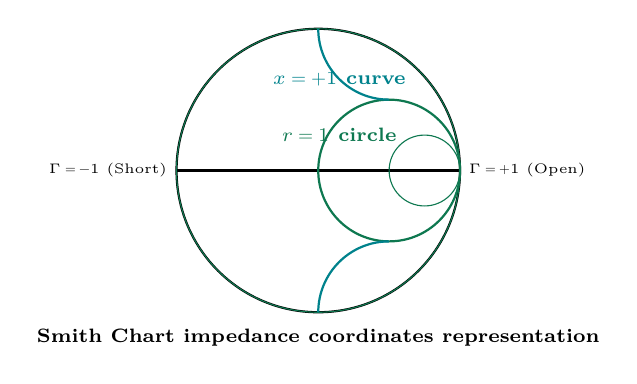
\begin{tikzpicture}[scale=0.9, every node/.style={font=\tiny}]
  % Outer boundary
  \draw[thick] (0,0) circle (2.0cm);
  
  % Real axis
  \draw[thick] (-2,0) -- (2,0);
  \node[left] at (-2,0) {$\Gamma = -1$ (Short)};
  \node[right] at (2,0) {$\Gamma = +1$ (Open)};
  
  % Constant Resistance circles (all touch (2,0))
  \draw[color=mygreen, thick] (1,0) circle (1.0cm); % r = 1
  \draw[color=mygreen, thin] (1.5,0) circle (0.5cm); % r = 3
  \draw[color=mygreen, thin] (0,0) circle (2.0cm); % r = 0 (same as boundary)
  
  % Constant Reactance curves
  % x = +1 curve
  \draw[color=myteal, thick] (1,1) arc (270:180:1.0cm);
  \draw[color=myteal, thick] (1,-1) arc (90:180:1.0cm);
  
  \node[color=mygreen, font=\scriptsize\bfseries] at (0.3,0.5) {$r=1$ circle};
  \node[color=myteal, font=\scriptsize\bfseries] at (0.3,1.3) {$x=+1$ curve};
  \node[below, font=\scriptsize\bfseries] at (0,-2.1) {Smith Chart impedance coordinates representation};
\end{tikzpicture}
\end{tcolorbox}

\subsection{Single-Stub Matching}
A single-stub tuner uses a shunt (or series) short- or open-circuited transmission line stub placed at a distance $d$ from the load to match a load impedance $Z_L$ to the line impedance $Z_0$.

\begin{tcolorbox}[tikzbox, title={Shunt Single-Stub Matching Network}]
\centering
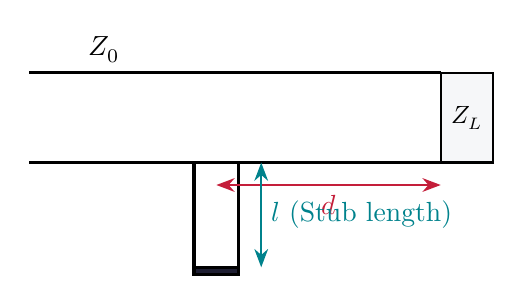
\begin{tikzpicture}[scale=0.95]
  % Main lines
  \draw[very thick] (0,0.6) -- (5.5,0.6);
  \draw[very thick] (0,-0.6) -- (5.5,-0.6);
  
  % Load box
  \draw[thick, fill=mygray] (5.5,-0.6) rectangle (6.2,0.6) node[midway, font=\small] {$Z_L$};
  
  % Shunt Stub (short-circuited at bottom)
  \draw[very thick] (2.2,-0.6) -- (2.2,-2.0);
  \draw[very thick] (2.8,-0.6) -- (2.8,-2.0);
  \draw[very thick, fill=mydark] (2.2,-2.0) rectangle (2.8,-2.1); % short circuit
  
  % Dimension arrows
  \draw[Stealth-Stealth, thick, color=myred] (2.5,-0.9) -- (5.5,-0.9) node[midway, below] {$d$};
  \draw[Stealth-Stealth, thick, color=myteal] (3.1,-0.6) -- (3.1,-2.0) node[midway, right] {$l$ (Stub length)};
  
  \node[above] at (1,0.6) {$Z_0$};
\end{tikzpicture}
\end{tcolorbox}

\subsubsection{Design Equations for Shunt Single-Stub}
Let $Y_L = 1/Z_L = G_L + j B_L$ be the load admittance. We normalize to $Y_0 = 1/Z_0$:
\begin{equation}
  y_L = g_L + j b_L = \frac{Y_L}{Y_0}
\end{equation}
The distance $d$ is chosen such that the admittance looking into the line at $d$ is:
\begin{equation}
  y_d = 1 + j b
\end{equation}
The stub length $l$ is then selected to provide a susceptance of $-j b$, canceling the reactive part and leaving a perfect match ($y_{\text{in}} = y_d + y_{\text{stub}} = 1$).
\begin{align}
  d &= \frac{\lambda}{2\pi} \tan^{-1}\left( \frac{r_L - 1}{x_L} \right) \quad (\text{simplified for specific cases}) \\
  l_s &= -\frac{\lambda}{2\pi} \tan^{-1}(b) \quad (\text{short-circuited stub})
\end{align}

% ===============================================================================
\section{Microwave Filter Design}
% ===============================================================================

Filters restrict frequencies allowed to pass. The modern \textbf{Insertion Loss Method} uses low-pass filter (LPF) prototypes with normalized values ($g_i$):
\begin{itemize}[leftmargin=*, itemsep=3pt]
  \item \textbf{Maximally Flat (Butterworth):} Flat passband response, roll-off is smooth.
  \item \textbf{Equal Ripple (Chebyshev):} Sharp cutoff, containing ripples in the passband.
\end{itemize}

\begin{tcolorbox}[formulabox, title={\textbf{Butterworth Prototype Values}}]
For a maximally flat low-pass filter, the element values $g_i$ ($1 \le i \le N$) are:
\begin{equation}
  g_i = 2 \sin \left[ \frac{(2i-1)\pi}{2N} \right] \quad \text{for } i = 1, 2, \dots, N
\end{equation}
And $g_{N+1} = 1.0$ for all $N$.
\end{tcolorbox}

% ===============================================================================
\section{RF and Microwave Amplifier Design}
% ===============================================================================

Microwave amplifier design utilizes active devices (transistors) characterized by their S-parameters:

\begin{tcolorbox}[tikzbox, title={Microwave Transistor Amplifier Block Diagram}]
\centering
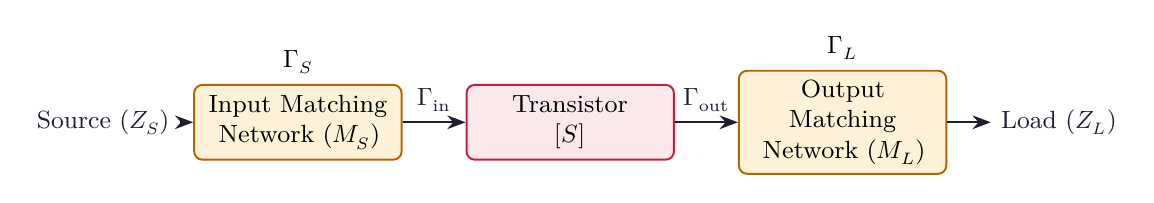
\begin{tikzpicture}[node distance=0.5cm and 0.8cm, every node/.style={font=\small}]
  \node[block, draw=myamber, fill=hdramber] (imn) {Input Matching\\Network ($M_S$)};
  \node[block, right=0.8cm of imn, draw=myred, fill=hdrred] (tx) {Transistor\\$[S]$};
  \node[block, right=0.8cm of tx, draw=myamber, fill=hdramber] (omn) {Output Matching\\Network ($M_L$)};
  
  \draw[arrow] (-1.5,0) node[left] {Source ($Z_S$)} -- (imn);
  \draw[arrow] (imn) -- (tx) node[midway, above] {$\Gamma_{\text{in}}$};
  \draw[arrow] (tx) -- (omn) node[midway, above] {$\Gamma_{\text{out}}$};
  \draw[arrow] (omn) -- (8.8,0) node[right] {Load ($Z_L$)};
  
  \node[above] at (imn.north) {$\Gamma_S$};
  \node[above] at (omn.north) {$\Gamma_L$};
\end{tikzpicture}
\end{tcolorbox}

\subsection{Amplifier Stability Criteria}
An amplifier is \textbf{unconditionally stable} if the transistor will not oscillate for any passive source and load impedance ($\text{Re}(Z_S), \text{Re}(Z_L) > 0$).
This requires the Rollett stability factor ($K$) to exceed 1 and the matrix determinant delta ($|\Delta|$) to be less than 1:

\begin{tcolorbox}[formulabox, title={\textbf{Rollett Stability Criteria}}]
\begin{align}
  K &= \frac{1 - |S_{11}|^2 - |S_{22}|^2 + |\Delta|^2}{2 |S_{12} S_{21}|} > 1 \\
  |\Delta| &= |S_{11}S_{22} - S_{12}S_{21}| < 1
\end{align}
If $K < 1$, the amplifier is only \textbf{conditionally stable}, and matching networks ($\Gamma_S, \Gamma_L$) must be chosen outside the unstable regions defined by the \textbf{stability circles}.
\end{tcolorbox}

\subsection{Amplifier Power Gains}
\begin{itemize}[leftmargin=*, itemsep=3pt]
  \item \textbf{Transducer Power Gain ($G_T$):} The ratio of power delivered to the load to the power available from the source.
    \begin{equation}
      G_T = \frac{1 - |\Gamma_S|^2}{|1 - S_{11}\Gamma_S|^2} |S_{21}|^2 \frac{1 - |\Gamma_L|^2}{|1 - S_{22}\Gamma_L - \frac{S_{12}S_{21}\Gamma_S\Gamma_L}{1 - S_{11}\Gamma_S}|^2}
    \end{equation}
  \item \textbf{Unilateral Transducer Gain ($G_{TU}$):} Assumes negligible feedback ($S_{12} = 0$).
    \begin{equation}
      G_{TU} = \frac{1 - |\Gamma_S|^2}{|1 - S_{11}\Gamma_S|^2} |S_{21}|^2 \frac{1 - |\Gamma_L|^2}{|1 - S_{22}\Gamma_L|^2}
    \end{equation}
\end{itemize}

\subsection{Low Noise Amplifier (LNA) Design \& Noise Figure Circles}
In LNA design (critical for receiver front-ends), the goal is to achieve the lowest possible Noise Figure ($F$), even at the expense of maximum transducer gain.
\begin{itemize}[leftmargin=*, itemsep=3pt]
  \item \textbf{Noise Figure Formula:}
    \begin{equation}
      F = F_{\text{min}} + \frac{4 R_n}{Z_0} \frac{|\Gamma_S - \Gamma_{\text{opt}}|^2}{(1 - |\Gamma_S|^2) |1 + \Gamma_{\text{opt}}|^2}
    \end{equation}
    where $F_{\text{min}}$ is the minimum noise figure of the transistor, $R_n$ is the equivalent noise resistance, $\Gamma_{\text{opt}}$ is the optimum source reflection coefficient, and $\Gamma_S$ is the actual source reflection coefficient.
  \item \textbf{Noise Figure Circles:} For a target noise figure $F > F_{\text{min}}$, the locus of all source reflection coefficients $\Gamma_S$ forms a circle on the Smith Chart.
    \begin{itemize}[leftmargin=*, itemsep=2.5pt, topsep=0pt]
      \item \textbf{Center ($C_F$):}
        \begin{equation}
          C_F = \frac{\Gamma_{\text{opt}}}{1 + N}
        \end{equation}
      \item \textbf{Radius ($R_F$):}
        \begin{equation}
          R_F = \frac{\sqrt{N^2 + N(1 - |\Gamma_{\text{opt}}|^2)}}{1 + N}
        \end{equation}
      \item \textbf{Noise Parameter ($N$):}
        \begin{equation}
          N = \frac{F - F_{\text{min}}}{4 R_n/Z_0} |1 + \Gamma_{\text{opt}}|^2
        \end{equation}
    \end{itemize}
    The designer selects a source reflection coefficient $\Gamma_S$ lying on the desired Noise Figure circle that offers a reasonable trade-off with input matching and gain.
\end{itemize}

% ===============================================================================
\section{Microwave Mixer Design}
% ===============================================================================

Mixers are 3-port non-linear devices that perform frequency translation by multiplying the RF input signal ($f_{\text{RF}}$) with a Local Oscillator signal ($f_{\text{LO}}$), producing an Intermediate Frequency ($f_{\text{IF}} = |f_{\text{RF}} \pm f_{\text{LO}}|$).
\begin{itemize}[leftmargin=*, itemsep=3pt]
  \item \textbf{Single-Ended Diode Mixer:} Uses a single Schottky diode. It is simple but provides poor isolation between the RF and LO ports, and does not suppress LO amplitude noise.
  \item \textbf{Balanced Mixer:} Utilizes two Schottky diodes combined via a 3 dB hybrid junction (such as a Magic Tee or branch-line coupler).
  \begin{itemize}[leftmargin=*, itemsep=2.5pt, topsep=0pt]
    \item \textbf{LO Noise Suppression:} The hybrid junction feeds the LO signal to the two diodes out-of-phase ($180^\circ$) while feeding the RF signal in-phase. The combined output at the IF port cancels out the LO amplitude noise.
    \item \textbf{Isolation:} Provides high isolation ($>20\,\text{dB}$) between the RF and LO ports, preventing local oscillator power leakage back into the antenna.
  \end{itemize}
  \item \textbf{Conversion Loss ($L_C$):} The ratio of RF input power to the desired IF output power:
    \begin{equation}
      L_C = 10 \log_{10}\left( \frac{P_{\text{RF}}}{P_{\text{IF}}} \right) \quad (\text{dB})
    \end{equation}
    For passive diode mixers, typical conversion loss ranges from $5\,\text{dB}$ to $8\,\text{dB}$.
\end{itemize}

% ===============================================================================
\section{Microwave Oscillator Design}
% ===============================================================================

Microwave oscillators convert DC power into RF power using active devices (transistors with positive feedback, or negative resistance diodes like Gunn and IMPATT).

\subsection{One-Port Negative Resistance Oscillator}
An active device presenting a negative input impedance $Z_{\text{in}} = R_{\text{in}} + j X_{\text{in}}$ (where $R_{\text{in}} < 0$) is terminated with a passive load impedance $Z_L = R_L + j X_L$:
\begin{itemize}[leftmargin=*, itemsep=3pt]
  \item \textbf{Startup Condition:} For oscillations to initiate from thermal noise:
    \begin{equation}
      R_{\text{in}} + R_L < 0 \quad \text{and} \quad X_{\text{in}} + X_L = 0
    \end{equation}
  \item \textbf{Steady-State Stability:} As the oscillation amplitude $A$ builds up, the negative resistance $R_{\text{in}}(A)$ saturates (becomes less negative) due to device non-linearities until a stable operating amplitude $A_0$ is reached:
    \begin{equation}
      R_{\text{in}}(A_0) + R_L = 0 \quad \text{and} \quad X_{\text{in}}(A_0) + X_L = 0
    \end{equation}
\end{itemize}

\subsection{Two-Port Transistor Oscillator}
A transistor-based oscillator uses an active three-terminal device (e.g., GaAs MESFET). An unstable termination at one port (such as a capacitive load at the source) is used to generate a negative input resistance at the other port (gate), which is then connected to a high-$Q$ resonant circuit (tuning network) to establish oscillation at the desired frequency.

\subsection{Microwave Power Amplifier Design}
Microwave power amplifiers (PAs) are designed to deliver high RF power levels to a load (typically a transmitting antenna) with maximum efficiency and minimal distortion.
\begin{itemize}[leftmargin=*, itemsep=3pt]
  \item \textbf{1-dB Compression Point ($P_{1\text{dB}}$):} As input power increases, the amplifier eventually saturates and gain drops. The $P_{1\text{dB}}$ is the power level at which the output power is $1\text{ dB}$ lower than it would be in the ideal linear region. It marks the boundary of the linear operating region.
  \item \textbf{Power Added Efficiency (PAE):} A critical metric for PAs that accounts for the input RF power, expressing the net RF power generated relative to the DC power consumed:
    \begin{equation}
      \text{PAE} = \frac{P_{\text{RF, out}} - P_{\text{RF, in}}}{P_{\text{DC}}} \times 100\%
    \end{equation}
  \item \textbf{Drain/Collector Efficiency ($\eta$):} Ratio of output RF power to input DC power: $\eta = P_{\text{RF, out}}/P_{\text{DC}} \times 100\%$.
\end{itemize}

\textbf{Power Amplifier Classes:}\par\noindent
PAs are classified based on their conduction angle ($\theta_c$), which defines the fraction of the RF cycle during which the active transistor conducts current.
\par\noindent
{\renewcommand{\arraystretch}{1.65}%
\begin{tabularx}{\linewidth}{|B{1.6cm}|Y|Y|Y|Y|}\hline
\textbf{Class} & \textbf{Conduction Angle ($\theta_c$)} & \textbf{Ideal Max Efficiency} & \textbf{Linearity} & \textbf{Characteristics} \\[4pt]
\hline
Class A & $360^\circ$ (conducts full cycle) & $50\%$ & Outstanding & Low efficiency; high heat dissipation; active at all times. \\[4pt]
\hline
Class AB & $180^\circ < \theta_c < 360^\circ$ & $50\% - 78.5\%$ & Good & Compromise between Class A and B; commonly used in RF links. \\[4pt]
\hline
Class B & $180^\circ$ (conducts half cycle) & $78.5\%$ & Moderate & Transistor conducts only during one half-cycle; requires push-pull. \\[4pt]
\hline
Class C & $<180^\circ$ (conducts narrow pulses) & $>85\%$ (approaching $100\%$) & Very Poor & High distortion; requires resonant tank circuit to reconstruct wave. \\[4pt]
\hline
\end{tabularx}
}

\begin{center}
  {\large\bfseries\color{myred} Quick Revision --- Module VI}\\[3pt]
  {\small\color{mydark} Microwave Design Principles $|$ PE-EC701A}
\end{center}
\noindent{\color{myred}\rule{\linewidth}{1.2pt}}
\vspace{4pt}

\begin{tcolorbox}[formulabox, title={\textbf{Key Formulas at a Glance}}]
\renewcommand{\arraystretch}{1.3}
\begin{tabularx}{\linewidth}{B{4.5cm} X}Rollett Stability factor & $K = \frac{1 - |S_{11}|^2 - |S_{22}|^2 + |\Delta|^2}{2|S_{12}S_{21}|}$ \\[4pt]
Determinant delta       & $\Delta = S_{11}S_{22} - S_{12}S_{21}$ \\[4pt]
Unilateral gain         & $G_{TU} = \frac{1-|\Gamma_S|^2}{|1-S_{11}\Gamma_S|^2} |S_{21}|^2 \frac{1-|\Gamma_L|^2}{|1-S_{22}\Gamma_L|^2}$ \\[4pt]
Butterworth filter      & $g_i = 2 \sin\left(\frac{(2i-1)\pi}{2N}\right)$ \\[4pt]
Unilateral figure merit  & $U = \frac{|S_{11}S_{12}S_{21}S_{22}|}{(1-|S_{11}|^2)(1-|S_{22}|^2)}$ \\[4pt]
LNA Noise Parameter ($N$) & $N = \frac{F - F_{\text{min}}}{4 R_n/Z_0} |1 + \Gamma_{\text{opt}}|^2$ \\[4pt]
LNA Circle Center ($C_F$) & $C_F = \frac{\Gamma_{\text{opt}}}{1 + N}$ \\[4pt]
LNA Circle Radius ($R_F$) & $R_F = \frac{\sqrt{N^2 + N(1 - |\Gamma_{\text{opt}}|^2)}}{1 + N}$
\end{tabularx}
\tcbset{colbacktitle=mygreen, coltitle=white}
\end{tcolorbox}

\begin{tcolorbox}[defbox, title={\textbf{One-Line Definitions}}]
\begin{itemize}[leftmargin=*, itemsep=2.5pt, topsep=0pt]
  \item \textbf{Smith Chart:} A graphical utility mapping reflection coefficients to complex impedances.
  \item \textbf{Stub Tuning:} Impedance matching using shunt or series transmission line segments.
  \item \textbf{Butterworth Filter:} A filter designed for a maximally flat amplitude response in the passband.
  \item \textbf{Chebyshev Filter:} A filter that provides sharp roll-off at the expense of equal-ripple passband ripples.
  \item \textbf{Rollett Stability:} Mathematical check ($K > 1$) determining if an amplifier is unconditionally stable.
  \item \textbf{LNA:} Low Noise Amplifier, designed to minimize noise figure circles on the input matching network.
  \item \textbf{Stability Circles:} Regions plotted on the Smith Chart enclosing unstable source/load reflection coefficients.
  \item \textbf{Conversion Loss:} The ratio of RF input power to IF output power in a passive mixer (expressed in dB).
  \item \textbf{Balanced Mixer:} A mixer using a hybrid junction to combine two diodes, canceling LO noise and providing port isolation.
  \item \textbf{One-Port Oscillator:} An oscillator designed by terminating a negative-resistance device with a resonant load.
\end{itemize}
\end{tcolorbox}

\begin{tcolorbox}[exambox, title={\textbf{Frequently Asked / Viva Questions}}]
\begin{enumerate}[topsep=0pt, label=\textbf{Q\arabic*.}, itemsep=5pt]
  \item \Q{What are constant resistance and constant reactance circles on a Smith Chart?}
    Constant resistance circles are circles whose centers lie on the horizontal real axis, all passing through the open-circuit point. Constant reactance circles are arcs representing imaginary parts.
  \item \Q{What is the difference between single-stub and double-stub matching?}
    Single-stub matching requires adjusting both the stub length and its position from the load. Double-stub matching uses fixed-position stubs, adjusting only their lengths.
  \item \Q{State the conditions for unconditional stability in microwave amplifiers.}
    The Rollett stability factor $K$ must be greater than 1 ($K > 1$) and the S-parameter determinant magnitude $|\Delta|$ must be less than 1 ($|\Delta| < 1$).
  \item \Q{Why are short-circuited stubs preferred over open-circuited stubs?}
    Because open-circuited stubs radiate energy from their open ends, behaving as antennas. Short-circuited stubs confine fields and are easier to manufacture with high precision.
  \item \Q{What is the unilateral assumption in amplifier design?}
    The assumption that $S_{12} = 0$, meaning there is no feedback from output to input. This simplifies the design of matching networks.
  \item \Q{Explain the insertion loss method of filter design.}
    It designs filters based on a power transfer function (like Butterworth or Chebyshev), yielding element values ($g_i$) normalized to a $1\,\Omega$ source and $1$ rad/s cutoff.
  \item \Q{What is the significance of Noise Figure Circles in LNA design?}
    They map the source reflection coefficients ($\Gamma_S$) that produce a constant noise figure, allowing the designer to balance noise figure and gain.
  \item \Q{Under what condition is single-stub matching not possible?}
    When the load impedance lies within a specific prohibited region of the Smith Chart (for a given shunt or series configuration), requiring a different stub location.
  \item \Q{What are Richards' Transformations?}
    Mathematical maps that convert lumped inductors and capacitors into transmission line stubs ($\text{L} \to \text{short stub}$, $\text{C} \to \text{open stub}$) at microwave frequencies.
  \item \Q{What is Kuroda's Identity?}
    A set of network equivalence rules used to separate filter stubs using redundant transmission line sections (unit elements).
  \item \Q{Explain the difference between power gain, available gain, and transducer gain.}
    Transducer gain accounts for mismatch at both input and output. Available gain assumes matched output. Power gain assumes matched input.
  \item \Q{What is the Unilateral Figure of Merit ($U$)?}
    A ratio used to calculate the maximum error introduced when assuming $S_{12} = 0$ instead of using the bilateral gain equations.
  \item \Q{State the startup and steady-state conditions for a negative resistance one-port oscillator.}
    Startup: $R_{\text{in}} + R_L < 0$ and $X_{\text{in}} + X_L = 0$ (net loop resistance is negative, allowing oscillations to build from thermal noise). Steady-state: $R_{\text{in}}(A_0) + R_L = 0$ and $X_{\text{in}}(A_0) + X_L = 0$ (saturation reduces negative resistance until net loop resistance is zero, sustaining a stable amplitude $A_0$).
  \item \Q{How does a balanced mixer achieve LO noise suppression?}
    By using a 3 dB hybrid junction (such as a Magic Tee) that feeds the local oscillator (LO) signal to the two diodes $180^\circ$ out-of-phase, while feeding the RF signal in-phase. The combined IF output cancels the LO amplitude noise components.
\end{enumerate}
\tcbset{colbacktitle=mgframe, coltitle=mydark}
\end{tcolorbox}

\begin{tcolorbox}[tikzbox, title={Comparison of Single-Stub and Double-Stub Tuning}]
\renewcommand{\arraystretch}{1.4}
\par\noindent
{\renewcommand{\arraystretch}{1.55}%
\begin{tabularx}{\linewidth}{|B{3.2cm}|Y|Y|}\hline
\textbf{Feature} & \textbf{\color{myteal}Single-Stub Tuning} & \textbf{\color{myamber}Double-Stub Tuning} \\[4pt]
\hline
\textbf{Stub Position} & Must be variable (requires sliding stub or custom line length). & Fixed spacing (typically $\lambda/8$ or $3\lambda/8$). \\[4pt]
\hline
\textbf{Adjustment} & Adjusts both stub length and stub distance from the load. & Adjusts only the lengths of the two stubs. \\[4pt]
\hline
\textbf{Matching Range} & Can match any load impedance with non-zero real part. & Cannot match all loads (contains a "forbidden region"). \\[4pt]
\hline
\textbf{Implementation} & Difficult in microstrip (requires changing physical layout). & Easy in microstrip (stubs are printed at fixed locations). \\[4pt]
\hline
\end{tabularx}
}
\end{tcolorbox}


% -- Module 7 -----------------------------------------------------------------
\modulestart{7}{Antenna Parameters}

\section{Antenna Parameters}
% ===============================================================================

Antennas are transitions between guided waves and free-space radiation. They are characterized by several fundamental parameters.

\begin{tcolorbox}[defbox]
\textbf{Effective Aperture ($A_e$):} A parameter describing the power-collecting ability of an antenna. It is the ratio of received power to the incident wave power density:
\begin{equation}
  A_e = \frac{P_{\text{rec}}}{W_i} \quad (\text{m}^2)
\end{equation}
\end{tcolorbox}

\begin{tcolorbox}[formulabox, title={\textbf{Core Antenna Parameters}}]
\begin{enumerate}[label=\textbf{\arabic*.}, leftmargin=1.5em, itemsep=4pt, topsep=2pt]
  \item \textbf{Directive Gain ($G_d$) \& Directivity ($D$):} Directivity is the maximum value of directive gain in the peak radiation direction.
    \begin{equation}
      D = \frac{4\pi U_{\text{max}}}{P_{\text{rad}}}
    \end{equation}
  \item \textbf{Aperture Gain Relation:}
    \begin{equation}
      G = D \cdot \eta_{\text{rad}} = \frac{4\pi A_e}{\lambda^2}
    \end{equation}
  \item \textbf{Beamwidth (HPBW \& FNBW):} Half-Power Beam Width (HPBW) is the angular span between the $3\text{ dB}$ down points. First-Null Beam Width (FNBW) is the span between the first zero-intensity nulls.
    \begin{equation}
      \text{FNBW} \approx 2 \times \text{HPBW}
    \end{equation}
\end{enumerate}
\end{tcolorbox}

% ===============================================================================
\section{Ground-Based Systems}
% ===============================================================================

\subsection{Horn Antenna}
Horn antennas flare the end of a waveguide to match the waveguide impedance to the intrinsic impedance of free space ($377\,\Omega$), minimizing reflection.

\begin{tcolorbox}[tikzbox, title={Horn Antenna Types}]
\centering
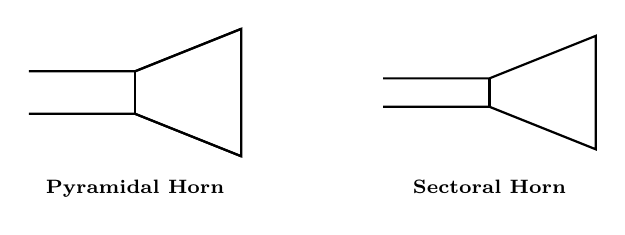
\begin{tikzpicture}[scale=0.9, every node/.style={font=\scriptsize}]
  % Pyramidal Horn (flared in both planes)
  \draw[thick] (0,0.3) -- (1.5,0.3) -- (3.0,0.9) -- (3.0,-0.9) -- (1.5,-0.3) -- (0,-0.3);
  \draw[thick] (1.5,0.3) -- (1.5,-0.3);
  \draw[thick] (3.0,0.9) -- (3.0,-0.9);
  \draw[thick] (1.5,0.3) -- (3.0,0.9);
  \draw[thick] (1.5,-0.3) -- (3.0,-0.9);
  \node[below, font=\scriptsize\bfseries] at (1.5,-1.1) {Pyramidal Horn};
  
  % Sectoral Horn
  \draw[thick] (5,0.2) -- (6.5,0.2) -- (8.0,0.8) -- (8.0,-0.8) -- (6.5,-0.2) -- (5,-0.2);
  \draw[thick] (6.5,0.2) -- (6.5,-0.2);
  \node[below, font=\scriptsize\bfseries] at (6.5,-1.1) {Sectoral Horn};
\end{tikzpicture}
\end{tcolorbox}

\textbf{Pyramidal Horn Gain:}
  \begin{equation}
    G = \frac{4\pi}{\lambda^2} \epsilon_{ap} A = \frac{4\pi}{\lambda^2} \epsilon_{ap} (a_e b_e)
  \end{equation}
  where $a_e, b_e$ are the aperture widths and $\epsilon_{ap}$ is the aperture efficiency.

\subsection{Parabolic Reflector Antenna}
Reflector antennas focus a feed horn's spherical wavefronts into highly directive plane waves.
\textbf{Cassegrain Feed:} Uses a primary parabolic reflector, a secondary hyperbolic sub-reflector at the focus, and a feed horn placed at the vertex of the primary dish.

\begin{tcolorbox}[tikzbox, title={Cassegrain Feed Ray-Tracing Geometry}]
\centering
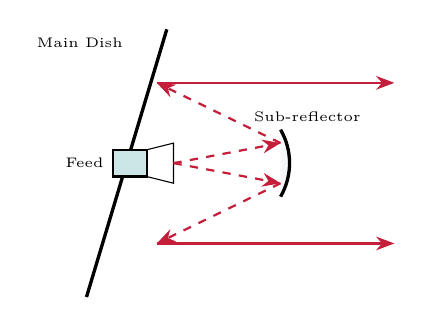
\begin{tikzpicture}[scale=0.85]
  % Main parabolic dish
  \draw[very thick, domain=-2:2, samples=50] plot (\x*0.3 - 0.5, \x);
  
  % Sub-reflector (hyperbolic)
  \draw[very thick, fill=mygray] (1.8,-0.5) arc (-30:30:1.0);
  
  % Feed horn at vertex
  \draw[thick, fill=myteal!20] (-0.7,-0.2) rectangle (-0.2,0.2);
  \draw (-0.2,0.2) -- (0.2,0.3) -- (0.2,-0.3) -- (-0.2,-0.2);
  \node[left, font=\tiny] at (-0.7,0) {Feed};
  
  % Ray tracing (horn -> sub-reflector -> dish -> out)
  \draw[arrow, color=myred, dashed] (0.2,0) -- (1.8,0.3);
  \draw[arrow, color=myred, dashed] (1.8,0.3) -- (-0.05, 1.2);
  \draw[arrow, color=myred] (-0.05, 1.2) -- (3.5, 1.2);
  
  \draw[arrow, color=myred, dashed] (0.2,0) -- (1.8,-0.3);
  \draw[arrow, color=myred, dashed] (1.8,-0.3) -- (-0.05, -1.2);
  \draw[arrow, color=myred] (-0.05, -1.2) -- (3.5, -1.2);
  
  \node[font=\tiny] at (2.2,0.7) {Sub-reflector};
  \node[font=\tiny] at (-1.2,1.8) {Main Dish};
\end{tikzpicture}
\end{tcolorbox}

\textbf{Gain:} $G = \left(\frac{\pi D}{\lambda}\right)^{\!2} \eta_{ap}$ where $D$ is the diameter of the dish.

% ===============================================================================
\section{Airborne and Planar Antennas}
% ===============================================================================

Airborne antennas must be aerodynamic, low-weight, and often conformal (matching the contour of the aircraft skin).

\subsection{Microstrip Patch Antenna}
A microstrip patch antenna consists of a radiating metallic patch printed on one side of a thin dielectric substrate with a continuous ground plane on the other.

\begin{tcolorbox}[tikzbox, title={Microstrip Patch Antenna Structure}]
\centering
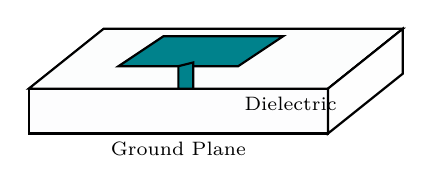
\begin{tikzpicture}[scale=0.95]
  % Substrate (3D-like box)
  \draw[thick, fill=mygray!30] (0,0) -- (4,0) -- (5,0.8) -- (1,0.8) -- cycle;
  \draw[thick, fill=mygray!20] (0,-0.6) -- (4,-0.6) -- (4,0) -- (0,0) -- cycle;
  \draw[thick, fill=mygray!10] (4,-0.6) -- (5,0.2) -- (5,0.8) -- (4,0) -- cycle;
  
  % Patch (printed on top of substrate)
  \draw[thick, fill=myteal] (1.2,0.3) -- (2.8,0.3) -- (3.4,0.7) -- (1.8,0.7) -- cycle;
  
  % Microstrip feed line
  \draw[thick, fill=myteal] (2.0,0) -- (2.0,0.3) -- (2.2,0.35) -- (2.2,0) -- cycle;
  
  % Labels
  \node[font=\scriptsize\color{myteal}] at (2.3,0.5) {Patch};
  \node[font=\scriptsize] at (3.5,-0.2) {Dielectric};
  \node[font=\scriptsize] at (2,-0.8) {Ground Plane};
\end{tikzpicture}
\end{tcolorbox}

\textbf{Feed Techniques:}
\begin{enumerate}[leftmargin=*, itemsep=3pt]
  \item \textbf{Microstrip Line Feed:} Easy to print, easy to match using inset cuts.
  \item \textbf{Coaxial Probe Feed:} Feed probe is connected through a hole from the bottom ground, matching is done by adjusting the insertion point.
  \item \textbf{Aperture-Coupled Feed:} Non-contact feed where a slot in the ground plane couples energy from a bottom line.
  \item \textbf{Proximity-Coupled Feed:} Multi-layer line printed directly below the patch.
\end{enumerate}

% ===============================================================================
% MANDATORY QUICK REVISION PAGE
% ===============================================================================
\newpage
\begin{center}
  {\large\bfseries\color{myred} Quick Revision --- Module VII}\\[3pt]
  {\small\color{mydark} Microwave Antennas $|$ PE-EC701A}
\end{center}
\noindent{\color{myred}\rule{\linewidth}{1.2pt}}
\vspace{4pt}

\begin{tcolorbox}[formulabox, title={\textbf{Key Formulas at a Glance}}]
\renewcommand{\arraystretch}{1.3}
\begin{tabularx}{\linewidth}{B{4.5cm} X}Effective Aperture      & $A_e = \frac{\lambda^2}{4\pi} G$ \\[4pt]
Horn Antenna Gain       & $G = \frac{4\pi}{\lambda^2} \epsilon_{ap} (a_e b_e)$ \\[4pt]
Parabolic Dish Gain     & $G = \left(\frac{\pi D}{\lambda}\right)^{\!2} \eta_{ap}$ \\[4pt]
Parabolic HPBW          & $\text{HPBW} \approx 70 \frac{\lambda}{D} \quad (\text{degrees})$ \\[4pt]
Patch Length            & $L \approx \frac{c}{2 f_0 \sqrt{\epsilon_{\text{eff}}}} - 2\Delta L$
\end{tabularx}
\tcbset{colbacktitle=mygreen, coltitle=white}
\end{tcolorbox}

\begin{tcolorbox}[defbox, title={\textbf{One-Line Definitions}}]
\begin{itemize}[leftmargin=*, itemsep=2.5pt, topsep=0pt]
  \item \textbf{Directivity:} The ratio of maximum radiation intensity to average radiation intensity.
  \item \textbf{Pyramidal Horn:} A waveguide flaring in both electric and magnetic field planes to match free space.
  \item \textbf{Cassegrain Feed:} A dual-reflector antenna utilizing a parabolic dish and a hyperbolic sub-reflector.
  \item \textbf{Aperture Efficiency:} The ratio of the effective antenna aperture to its physical geometric area.
  \item \textbf{Polarization:} The orientation of the electric field vector of the radiated wave as it propagates.
  \item \textbf{Conformal Antenna:} An antenna designed to follow the curved contour of an host aircraft or vehicle.
  \item \textbf{Aperture Coupling:} A non-contact microstrip feeding technique using a slot in a shared ground plane.
\end{itemize}
\end{tcolorbox}

\begin{tcolorbox}[exambox, title={\textbf{Frequently Asked / Viva Questions}}]
\begin{enumerate}[topsep=0pt, label=\textbf{Q\arabic*.}, itemsep=5pt]
  \item \Q{State the relation between antenna gain, directivity, and efficiency.}
    $G = \eta_{\text{rad}} \cdot D$, where $\eta_{\text{rad}}$ is the radiation efficiency. For a lossless antenna, gain equals directivity ($G = D$).
  \item \Q{What are the advantages of Cassegrain feeds over focal-point feeds?}
    Shorter waveguide feed lines (reducing insertion loss), lower spillover noise from the ground, and easier access to the feed horn at the vertex.
  \item \Q{Explain the physical operation of a microstrip patch antenna.}
    The patch acts as a resonant cavity. Radiation occurs primarily from the fringing fields at the open-circuited edges of the patch.
  \item \Q{Why does flaring a waveguide into a horn antenna increase directivity?}
    Flaring increases the physical aperture area of the waveguide. Since $D \propto A/\lambda^2$, a larger aperture yields higher directivity and narrower beamwidth.
  \item \Q{What is circular polarization and when is it preferred?}
    A wave polarization where the E-field vector rotates in a circle. It is preferred in satellite links because it is immune to Faraday rotation in the ionosphere.
  \item \Q{Why do planar antennas require low-profile feed techniques in airborne systems?}
    To maintain aerodynamic properties, preventing wind drag, turbulence, and structural damage to the aircraft.
  \item \Q{State the difference between E-plane and H-plane sectoral horns.}
    An E-plane horn flares only in the direction of the electric field. An H-plane horn flares only in the direction of the magnetic field.
  \item \Q{How does the dielectric substrate thickness affect microstrip patch performance?}
    Thicker substrates increase bandwidth and radiation efficiency but lead to surface-wave excitation, causing radiation pattern degradation.
  \item \Q{What is FNBW and how is it related to HPBW?}
    FNBW is First-Null Beamwidth. For symmetric main lobes, FNBW is approximately twice the HPBW ($\text{FNBW} \approx 2 \times \text{HPBW}$).
  \item \Q{What is the purpose of the sub-reflector in a Cassegrain antenna?}
    To reflect the feed signals onto the main dish, allowing the feed electronics to be placed behind the main dish rather than suspended at the focus.
  \item \Q{How do lens antennas work at microwave frequencies?}
    They use dielectric materials to collimate spherical wavefronts into plane waves, similar to optical lenses.
  \item \Q{What is the typical gain range of a standard horn antenna?}
    Typically between $10\text{ dB}$ and $25\text{ dB}$, depending on flaring and operating frequency.
\end{enumerate}
\tcbset{colbacktitle=mgframe, coltitle=mydark}
\end{tcolorbox}

\begin{tcolorbox}[tikzbox, title={Comparison of Microwave Antennas}]
\renewcommand{\arraystretch}{1.4}
\par\noindent
{\renewcommand{\arraystretch}{1.55}%
\begin{tabularx}{\linewidth}{|B{3.0cm}|Y|Y|Y|}\hline
\textbf{Antenna Type} & \textbf{Typical Gain} & \textbf{Bandwidth} & \textbf{Physical Profile} \\
\hline
\textbf{Horn Antenna} & Moderate ($12 - 25$ dBi) & Wide (waveguide range) & Bulky flared structure \\[4pt]
\hline
\textbf{Parabolic Dish} & Very High ($30 - 50$ dBi) & Wide & Very bulky reflector assembly \\
\hline
\textbf{Microstrip Patch} & Low ($5 - 8$ dBi) & Very Narrow ($2\% - 5\%$) & Flat, lightweight, conformal \\[4pt]
\hline
\textbf{Lens Antenna} & High ($20 - 30$ dBi) & Moderate & Heavy dielectric component \\
\hline
\end{tabularx}
}
\end{tcolorbox}


% -- Module 8 -----------------------------------------------------------------
\modulestart{8}{Power Measurement}

\section{Power Measurement}
% ===============================================================================

Microwave power is categorized based on intensity levels: Low Power ($< 10$ mW), Medium Power (10 mW -- 10 W), and High Power ($> 10$ W).

\subsection{Bolometer Mount Method (Low Power)}
A bolometer is a temperature-sensitive resistor whose resistance changes when it absorbs RF power.
\begin{itemize}[leftmargin=*, itemsep=3pt]
  \item \textbf{Thermistor:} Has a \textbf{negative temperature coefficient (NTC)}; resistance decreases as temperature rises.
  \item \textbf{Barretter:} Has a \textbf{positive temperature coefficient (PTC)}; resistance increases as temperature rises.
\end{itemize}
The bolometer is placed in an active arm of a self-balancing Wheatstone bridge. The DC bias power required to balance the bridge is measured before and after applying RF power:
\begin{equation}
  P_{\text{RF}} = P_{\text{bias,1}} - P_{\text{bias,2}}
\end{equation}

\subsection{Calorimetric Method (High Power)}
High power is measured by absorbing the RF energy in a fluid load (usually water) and measuring the temperature rise ($\Delta T = T_{\text{out}} - T_{\text{in}}$).
\begin{equation}
  P_{\text{RF}} = \dot{m} C_p \Delta T
\end{equation}
where $\dot{m}$ is mass flow rate and $C_p$ is specific heat.

% ===============================================================================
\section{Impedance and Frequency Measurement}
% ===============================================================================

\subsection{Slotted Line Probe Technique}
A slotted line is a section of coaxial line or waveguide containing an axial slot that allows a small capacitive probe to slide along the length to sample the electric field.

\begin{tcolorbox}[tikzbox, title={Slotted Line Probe Mechanism}]
\centering
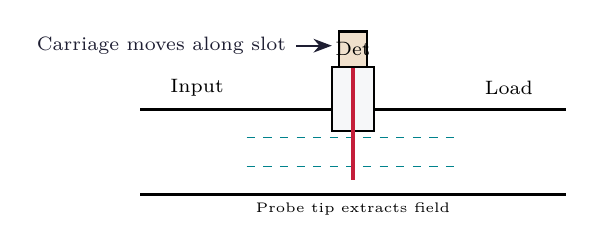
\begin{tikzpicture}[scale=0.9, every node/.style={font=\scriptsize}]
  % Waveguide segment
  \draw[very thick] (0,0.6) -- (6,0.6);
  \draw[very thick] (0,-0.6) -- (6,-0.6);
  
  % Slot representation (dashed lines)
  \draw[dashed, color=myteal] (1.5,0.2) -- (4.5,0.2);
  \draw[dashed, color=myteal] (1.5,-0.2) -- (4.5,-0.2);
  
  % Slide probe carriage
  \draw[thick, fill=mygray] (2.7,0.3) rectangle (3.3,1.2);
  \draw[line width=1.5pt, color=myred] (3.0, 1.2) -- (3.0, -0.4); % Probe tip
  
  % Crystal detector block on top
  \draw[thick, fill=myamber!20] (2.8,1.2) rectangle (3.2,1.7) node[midway] {Det};
  
  \node at (0.8,0.9) {Input};
  \node at (5.2,0.9) {Load};
  \node[font=\tiny] at (3.0, -0.8) {Probe tip extracts field};
  \draw[arrow] (2.2, 1.5) node[left] {Carriage moves along slot} -- (2.7, 1.5);
\end{tikzpicture}
\end{tcolorbox}

\begin{itemize}[leftmargin=*, itemsep=3pt]
  \item \textbf{Low VSWR Measurement ($1 < S < 10$):} Measured directly as the ratio of maximum to minimum probe outputs:
    \begin{equation}
      S = \frac{V_{\text{max}}}{V_{\text{min}}}
    \end{equation}
  \item \textbf{High VSWR Measurement (Double-Minimum Method, $S > 10$):}
    For high reflection, the minimum is sharp and close to the noise floor. We measure the distance $\Delta x$ between two positions where output power is twice the minimum value:
    \begin{equation}
      S = \frac{\lambda_g}{\pi \Delta x}
    \end{equation}
\end{itemize}

% ===============================================================================
\section{Vector Network Analyzer (VNA)}
% ===============================================================================

A Vector Network Analyzer measures the complete S-parameters (both magnitude and phase) of a device under test (DUT) by separating incident, reflected, and transmitted waves.

\begin{tcolorbox}[tikzbox, title={Vector Network Analyzer Simplified Architecture}]
\centering
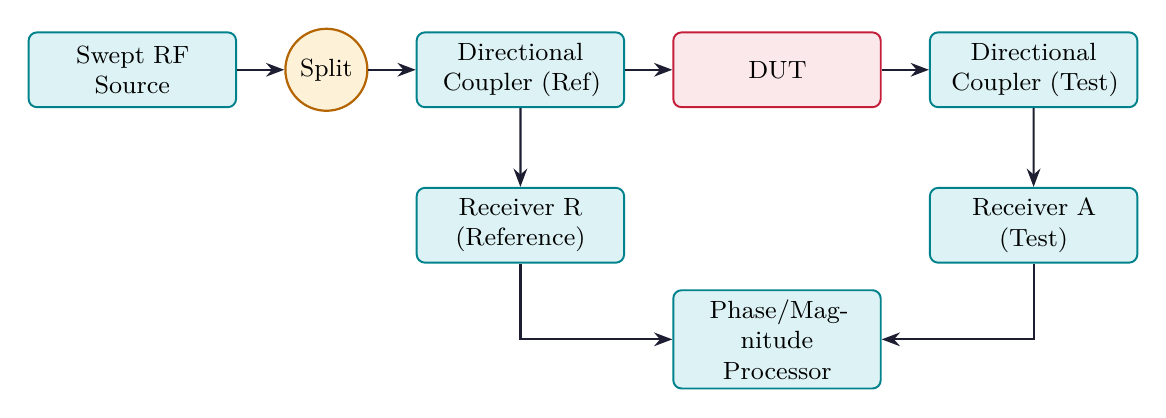
\begin{tikzpicture}[scale=0.9, every node/.style={font=\scriptsize}]
  \node[block] (src) {Swept RF\\Source};
  \node[sumjunc, right=0.6cm of src] (div) {Split};
  \node[block, right=0.6cm of div] (coup1) {Directional\\Coupler (Ref)};
  \node[block, right=0.6cm of coup1, draw=myred, fill=hdrred] (dut) {DUT};
  \node[block, right=0.6cm of dut] (coup2) {Directional\\Coupler (Test)};
  
  \node[block, below=1.0cm of coup1] (rec1) {Receiver R\\(Reference)};
  \node[block, below=1.0cm of coup2] (rec2) {Receiver A\\(Test)};
  
  \node[block, below=2.3cm of dut] (dsp) {Phase/Magnitude\\Processor};
  
  \draw[arrow] (src) -- (div);
  \draw[arrow] (div) -- (coup1);
  \draw[arrow] (coup1) -- (dut);
  \draw[arrow] (dut) -- (coup2);
  
  \draw[arrow] (coup1) -- (rec1);
  \draw[arrow] (coup2) -- (rec2);
  
  \draw[arrow] (rec1.south) |- (dsp.west);
  \draw[arrow] (rec2.south) |- (dsp.east);
\end{tikzpicture}
\end{tcolorbox}

\textbf{Calibration:} System errors are calibrated out using the \textbf{SOLT} (Short, Open, Load, Thru) standard calibration procedure.

% ===============================================================================
\section{Spectrum Analyzer}
% ===============================================================================

A Spectrum Analyzer displays signal amplitude versus frequency, identifying harmonics, distortion, and noise floors.

\begin{tcolorbox}[tikzbox, title={Superheterodyne Spectrum Analyzer Block Diagram}]
\centering
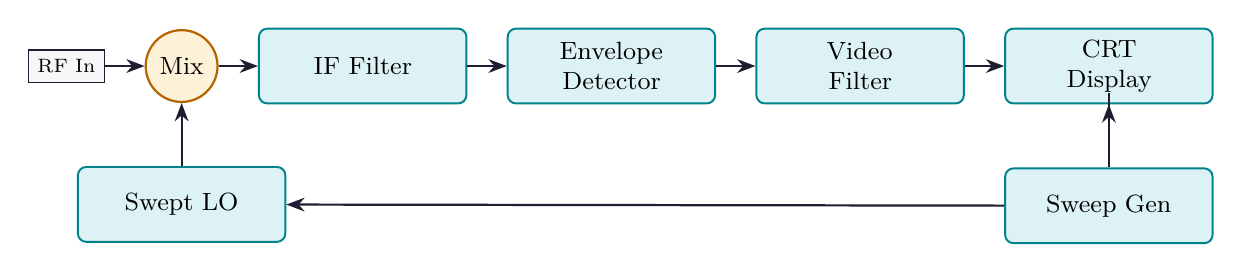
\begin{tikzpicture}[node distance=0.2cm and 0.5cm, every node/.style={font=\scriptsize}]
  \node[draw=mydark, fill=mygray, minimum size=0.4cm] (in) {RF In};
  \node[sumjunc, right=0.5cm of in] (mix) {Mix};
  \node[block, right=0.5cm of mix] (if) {IF Filter};
  \node[block, right=0.5cm of if] (det) {Envelope\\Detector};
  \node[block, right=0.5cm of det] (vid) {Video\\Filter};
  \node[block, right=0.5cm of vid] (crt) {CRT\\Display};
  
  \node[block, below=0.8cm of mix] (lo) {Swept LO};
  \node[block, below=0.8cm of crt] (swp) {Sweep Gen};
  
  \draw[arrow] (in) -- (mix);
  \draw[arrow] (mix) -- (if);
  \draw[arrow] (if) -- (det);
  \draw[arrow] (det) -- (vid);
  \draw[arrow] (vid) -- (crt);
  \draw[arrow] (lo) -- (mix);
  \draw[arrow] (swp) -- (lo);
  \draw[arrow] (swp) |- (crt.south);
\end{tikzpicture}
\end{tcolorbox}

% ===============================================================================
\section{Noise Measurement: Y-Factor Method}
% ===============================================================================

The Y-factor method is the standard technique for measuring the noise figure ($F$) of a receiver:

\begin{tcolorbox}[formulabox, title={\textbf{Y-Factor Method Equations}}]
We measure output noise power with a hot noise source at temperature $T_h$ and a cold noise source at temperature $T_c$. The ratio is:
\begin{equation}
  Y = \frac{N_{\text{hot}}}{N_{\text{cold}}} = \frac{T_h + T_e}{T_c + T_e}
\end{equation}
Solving for the equivalent noise temperature $T_e$ of the receiver:
\begin{equation}
  T_e = \frac{T_h - Y T_c}{Y - 1} \quad (\text{K})
\end{equation}
The noise figure $F$ is then calculated as:
\begin{equation}
  F = 1 + \frac{T_e}{T_0} \quad (\text{with } T_0 = 290\text{ K})
\end{equation}
\end{tcolorbox}

% ===============================================================================
\section{Measurement of Microwave Antenna Parameters}
% ===============================================================================

Antenna parameter measurements are critical for validating design parameters such as radiation pattern and directive gain.

\subsection{Radiation Pattern Measurement}
The radiation pattern is measured in the far-field region to ensure that the wave behaves as a local plane wave.
\begin{itemize}[leftmargin=*, itemsep=3pt]
  \item \textbf{Far-Field Boundary (Fraunhofer Distance):} The minimum distance $R$ between the transmitting antenna and the antenna under test (AUT) of maximum dimension $D$ is:
    \begin{equation}
      R \ge \frac{2 D^2}{\lambda} \quad (\text{m})
    \end{equation}
  \item \textbf{Setup:} Carried out in an \textbf{anechoic chamber} lined with RF-absorbing foam pyramids to eliminate echoes. The AUT is placed on a rotating positioner as a receiver, and a stationary source antenna transmits a signal. The received power is recorded as a function of the rotation angle ($\theta, \phi$) to plot the 2D/3D radiation pattern.
\end{itemize}

\subsection{Antenna Gain Measurement}
Gain is measured using either absolute or relative methods:
\begin{enumerate}[leftmargin=*, itemsep=3pt]
  \item \textbf{Three-Antenna Method (Absolute Method):} Requires no prior knowledge of any antenna's gain. By measuring the received power combinations ($P_{ij}$) among three different antennas ($A, B, C$) separated by distance $R$, we apply the \textbf{Friis Transmission Equation} to solve for individual gains:
    \begin{equation}
      G_i G_j = \left( \frac{4\pi R}{\lambda} \right)^{\!2} \frac{P_{rec, j}}{P_{trans, i}}
    \end{equation}
    Taking the logarithm yields a system of three linear equations to find $G_A, G_B, G_C$.
  \item \textbf{Gain Transfer Method (Comparison Method):} The received power of a standard gain horn antenna (with known gain $G_{std}$) is measured first as $P_{std}$. The AUT is then substituted in the exact same position, and its received power $P_{AUT}$ is measured. The gain of the AUT is calculated as:
    \begin{equation}
      G_{AUT} = G_{std} \cdot \frac{P_{AUT}}{P_{std}} \quad \implies \quad G_{AUT (dBi)} = G_{std (dBi)} + 10 \log_{10}\left(\frac{P_{AUT}}{P_{std}}\right)
    \end{equation}
\end{enumerate}

% ===============================================================================
% MANDATORY QUICK REVISION PAGE
% ===============================================================================
\newpage
\begin{center}
  {\large\bfseries\color{myred} Quick Revision --- Module VIII}\\[3pt]
  {\small\color{mydark} Microwave Measurements $|$ PE-EC701A}
\end{center}
\noindent{\color{myred}\rule{\linewidth}{1.2pt}}
\vspace{4pt}

\begin{tcolorbox}[formulabox, title={\textbf{Key Formulas at a Glance}}]
\renewcommand{\arraystretch}{1.3}
\begin{tabularx}{\linewidth}{B{4.5cm} X}Low VSWR                & $S = \frac{V_{\text{max}}}{V_{\text{min}}}$ \\[4pt]
Double-Minimum VSWR     & $S = \frac{\lambda_g}{\pi \Delta x}$ \quad ($\Delta x$ is distance between $2V_{\text{min}}$ points) \\[4pt]
Calorimetric Power      & $P = \dot{m} C_p (T_{\text{out}} - T_{\text{in}})$ \\[4pt]
Y-Factor Relation       & $Y = \frac{N_{\text{hot}}}{N_{\text{cold}}} = \frac{T_h+T_e}{T_c+T_e}$ \\[4pt]
Receiver Noise Temp     & $T_e = \frac{T_h - Y T_c}{Y - 1}$
\end{tabularx}
\tcbset{colbacktitle=mygreen, coltitle=white}
\end{tcolorbox}

\begin{tcolorbox}[defbox, title={\textbf{One-Line Definitions}}]
\begin{itemize}[leftmargin=*, itemsep=2.5pt, topsep=0pt]
  \item \textbf{Thermistor:} A temperature-sensitive resistor with a negative temperature coefficient (NTC).
  \item \textbf{Barretter:} A thin platinum wire bolometer element with a positive temperature coefficient (PTC).
  \item \textbf{Slotted Line:} A waveguide with an axial slot used to sample electric field standing wave patterns.
  \item \textbf{VNA:} An instrument that measures the amplitude and phase of reflection/transmission S-parameters.
  \item \textbf{Spectrum Analyzer:} A swept receiver displaying power spectral density versus frequency.
  \item \textbf{Y-Factor:} The ratio of receiver output noise powers under hot and cold source excitations.
  \item \textbf{SOLT Calibration:} Standard VNA calibration using Short, Open, Load, and Thru reference elements.
\end{itemize}
\end{tcolorbox}

\begin{tcolorbox}[exambox, title={\textbf{Frequently Asked / Viva Questions}}]
\begin{enumerate}[topsep=0pt, label=\textbf{Q\arabic*.}, itemsep=5pt]
  \item \Q{Explain why a bolometer Wheatstone bridge must be self-balancing.}
    Applying RF power heats the bolometer, changing its resistance and unbalancing the bridge. Automatically reducing DC bias to re-balance the bridge allows RF power to be measured from the DC power difference, keeping bolometer resistance constant.
  \item \Q{What is the double-minimum method and when is it used?}
    It is a method to measure high VSWR ($S > 10$). We measure the distance $\Delta x$ between the $3\text{ dB}$ points around a standing-wave minimum. It is used because direct $V_{\text{max}}/V_{\text{min}}$ measurements are inaccurate near the noise floor.
  \item \Q{What is the difference between a scalar and a vector network analyzer?}
    A Scalar Network Analyzer (SNA) only measures amplitude transmission and reflection coefficients. A Vector Network Analyzer (VNA) measures both amplitude and phase.
  \item \Q{Why does a frequency wavemeter have a resonant cavity?}
    It is a tunable cavity resonator. When tuned to the input frequency, it absorbs a fraction of power, creating a dip in the through-line power meter to indicate frequency.
  \item \Q{Explain the SOLT calibration method.}
    VNA calibration standards: Short circuit (reflects phase $180^\circ$), Open circuit (reflects phase $0^\circ$), matched Load (absorbs all power), and Thru connection (connects ports directly).
  \item \Q{Describe the basic block diagram of a superheterodyne spectrum analyzer.}
    RF input is mixed with a swept LO. The resulting IF signal is filtered, envelope-detected, and displayed on a screen swept in sync with the LO.
  \item \Q{How is antenna gain measured using the comparison method?}
    The received power of a standard gain horn (known gain $G_s$) is measured. The test antenna is then substituted, and its received power $P_t$ is measured. The test gain is $G_t = G_s (P_t/P_s)$.
  \item \Q{Why is calorimetric power measurement used for high powers?}
    Because solid-state sensors (bolometers/diodes) saturate or burn out at high powers. Fluid loads can absorb kilowatts of power safely, converting it to measurable heat.
  \item \Q{What is the physical meaning of the equivalent noise temperature ($T_e$)?}
    It is the temperature of a dummy resistor at the input of an ideal noiseless receiver that would generate the same noise power as the actual noisy receiver.
  \item \Q{Why is the slot in a slotted line waveguide cut along the center of the broad wall?}
    Because the slot is parallel to the surface current flow lines of the dominant $\text{TE}_{10}$ mode. This minimizes field distortion and leakage.
  \item \Q{What are the typical noise sources used in Y-factor measurements?}
    Gas discharge tubes or avalanche diodes that can switch between a room temperature state (cold) and a high electron temperature state (hot).
  \item \Q{How does a Spectrum Analyzer differ from an Oscilloscope?}
    An oscilloscope displays signal amplitude versus time (time domain). A spectrum analyzer displays signal amplitude versus frequency (frequency domain).
\end{enumerate}
\tcbset{colbacktitle=mgframe, coltitle=mydark}
\end{tcolorbox}

\begin{tcolorbox}[tikzbox, title={Comparison of VNA and Spectrum Analyzer}]
\renewcommand{\arraystretch}{1.4}
\par\noindent
{\renewcommand{\arraystretch}{1.65}%
\begin{tabularx}{\linewidth}{|B{3.0cm}|Y|Y|}\hline
\textbf{Feature} & \textbf{Vector Network Analyzer (VNA)} & \textbf{Spectrum Analyzer} \\
\hline
\textbf{Signal Source} & Built-in swept source (active stimulus). & None (passive measurement of external signal). \\[4pt]
\hline
\textbf{Quantities Measured} & S-parameters ($S_{11}, S_{21}$, etc.), phase, group delay. & Frequency component amplitudes, harmonics, noise floor. \\[4pt]
\hline
\textbf{Calibration} & Extremely complex (SOLT calibration required). & Simple amplitude calibration. \\[4pt]
\hline
\textbf{Primary Use} & Characterizing passive/active components (filters, antennas). & Analyzing transmitter signals, interference, distortion. \\[4pt]
\hline
\end{tabularx}
}
\end{tcolorbox}


% -- Module 9 -----------------------------------------------------------------
\modulestart{9}{Radar Systems}

\section{Radar Systems}
% ===============================================================================

RADAR (RAdio Detection And Ranging) is an active electromagnetic system that transmits microwave pulses and processes reflections to determine target range, velocity, and angle.

\begin{tcolorbox}[tikzbox, title={Pulsed Radar Block Diagram}]
\centering
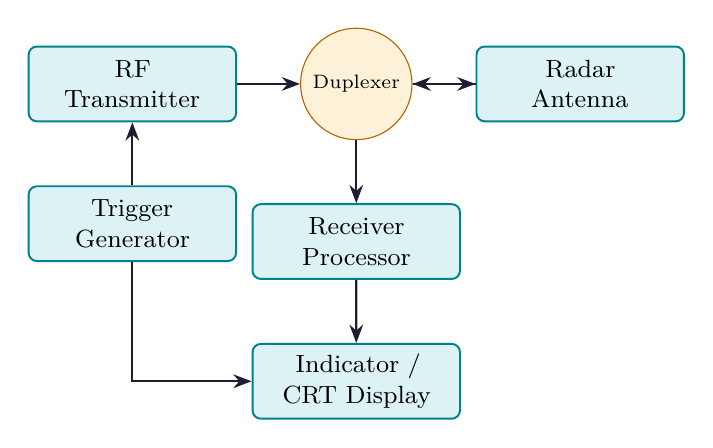
\begin{tikzpicture}[scale=0.9, every node/.style={font=\scriptsize}]
  \node[block] (tx) {RF\\Transmitter};
  \node[block, below=0.8cm of tx] (trg) {Trigger\\Generator};
  \node[circle, draw=myamber, fill=hdramber, right=0.8cm of tx, minimum size=0.8cm] (dup) {Duplexer};
  \node[block, right=0.8cm of dup] (ant) {Radar\\Antenna};
  \node[block, below=0.8cm of dup] (rx) {Receiver\\Processor};
  \node[block, below=0.8cm of rx] (dsp) {Indicator /\\CRT Display};
  
  \draw[arrow] (tx) -- (dup);
  \draw[arrow] (dup) -- (ant);
  \draw[arrow] (ant) -- (dup); % Return path
  \draw[arrow] (dup) -- (rx);
  
  \draw[arrow] (trg) -- (tx);
  \draw[arrow] (trg) |- (dsp);
  \draw[arrow] (rx) -- (dsp);
\end{tikzpicture}
\end{tcolorbox}

\begin{tcolorbox}[formulabox, title={\textbf{Radar Range Equation}}]
The maximum radar detection range $R_{\text{max}}$ is given by:
\begin{equation}
  R_{\text{max}} = \left[ \frac{P_t G^2 \lambda^2 \sigma}{(4\pi)^3 P_{\text{min}}} \right]^{\!1/4} \quad (\text{m})
\end{equation}
Where:
\begin{itemize}[leftmargin=1.5em, itemsep=1pt, topsep=2pt]
  \item[] $P_t$ = peak transmitter power (W)
  \item[] $G$ = antenna gain
  \item[] $\lambda$ = RF operating wavelength (m)
  \item[] $\sigma$ = Radar Cross Section (RCS) of target ($\text{m}^2$)
  \item[] $P_{\text{min}}$ = minimum detectable receiver signal (W)
\end{itemize}
\end{tcolorbox}

\textbf{Radar Variations:}
\begin{enumerate}[leftmargin=*, itemsep=3pt]
  \item \textbf{CW (Continuous Wave) Radar:} Transmits continuously, measures velocity using \textbf{Doppler shift} ($f_d = 2v/\lambda$).
  \item \textbf{FMCW (Frequency Modulated CW) Radar:} Sweeps transmitter frequency, allowing both range and velocity to be measured.
  \item \textbf{MTI (Moving Target Indicator) Radar:} Suppresses static clutter (ground, buildings) using delay-line cancelers.
\end{enumerate}

% ===============================================================================
\section{Terrestrial and Satellite Communications}
% ===============================================================================

\begin{tcolorbox}[tikzbox, title={Satellite Uplink/Downlink Path Schematic}]
\centering
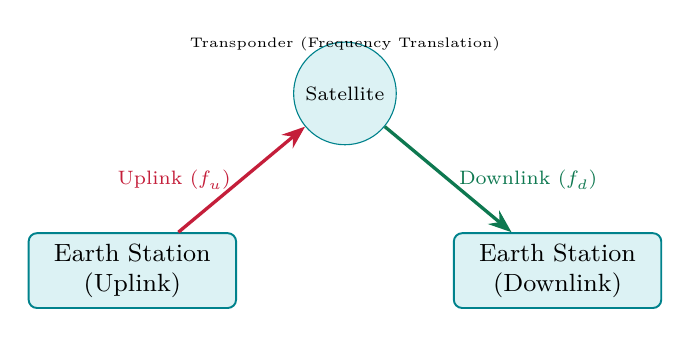
\begin{tikzpicture}[scale=0.9, every node/.style={font=\scriptsize}]
  \node[draw=myteal, fill=hdrteal, circle, minimum size=1.0cm] (sat) at (3,2.5) {Satellite};
  \node[block] (es1) at (0,0) {Earth Station\\(Uplink)};
  \node[block] (es2) at (6,0) {Earth Station\\(Downlink)};
  
  \draw[arrow, color=myred, line width=1.2pt] (es1) -- (sat) node[midway, left] {Uplink ($f_u$)};
  \draw[arrow, color=mygreen, line width=1.2pt] (sat) -- (es2) node[midway, right] {Downlink ($f_d$)};
  
  \node[font=\tiny] at (3, 3.2) {Transponder (Frequency Translation)};
\end{tikzpicture}
\end{tcolorbox}

\textbf{Link Budget ($C/N$):} Carrier-to-Noise ratio at the receiver terminal:
  \begin{equation}
    \left(\frac{C}{N}\right)_{\text{dB}} = \text{EIRP}_{\text{dBW}} + \left(\frac{G}{T}\right)_{\text{dB/K}} - \text{FSL}_{\text{dB}} - k_{\text{dBW}} - B_{\text{dB-Hz}}
  \end{equation}
  where $\text{EIRP}$ is Equivalent Isotropic Radiated Power, $G/T$ is receiver figure of merit, $\text{FSL} = (4\pi d/\lambda)^2$ is Free Space Path Loss, and $k$ is Boltzmann's constant.

% ===============================================================================
\section{Radio Aids to Navigation}
% ===============================================================================

\begin{itemize}[leftmargin=*, itemsep=3pt]
  \item \textbf{GPS (Global Positioning System):} Employs 24+ satellites. Receivers measure transit times of signals from 4+ satellites, using \textbf{triangulation} to resolve latitude, longitude, altitude, and clock bias.
  \item \textbf{ILS (Instrument Landing System):} Provides guidance for aircraft landing: \textbf{Localizer} (lateral guidance, 108--112 MHz) and \textbf{Glide Slope} (vertical guidance, 329--335 MHz).
  \item \textbf{LORAN (Long Range Navigation):} Hyperbolic radio navigation system using time-difference arrivals of pulses from ground stations.
  \item \textbf{RFID (Radio Frequency Identification):} Uses electromagnetic coupling in microwave/RF bands for asset tracking.
\end{itemize}

% ===============================================================================
\section{Modern Trends: Biological Effects, MMICs, and RFMEMS}
% ===============================================================================

\begin{itemize}[leftmargin=*, itemsep=3pt]
  \item \textbf{Biological Effects \& SAR:} Microwaves cause dielectric heating of tissues. The \textbf{SAR (Specific Absorption Rate)} measures RF energy absorption by body tissues:
    \begin{equation}
      \text{SAR} = \frac{\sigma |E|^2}{\rho} \quad (\text{W/kg})
    \end{equation}
    where $\sigma$ is tissue conductivity, $E$ is electric field, and $\rho$ is mass density. Regulatory limits are typically $1.6\text{ W/kg}$ over $1\text{ g}$ of tissue.
  \item \textbf{MMICs:} Monolithic Microwave Integrated Circuits integrate passive components, transmission lines, and active transistors onto a single semiconductor substrate (GaAs, GaN, SiGe).
  \item \textbf{RFMEMS:} Micro-Electro-Mechanical Systems designed for RF/microwave signals. They offer high isolation, low insertion loss, and low power consumption.
  \item \textbf{Microwave Imaging:} A non-invasive imaging technique that maps the spatial distribution of dielectric properties (permittivity and conductivity) inside a body.
  \begin{itemize}[leftmargin=*, itemsep=2.5pt, topsep=0pt]
    \item \textbf{Active Imaging (Radar-based):} Transmits low-power microwave pulses and records the backscattered signals to reconstruct a 3D profile of dielectric contrasts.
    \item \textbf{Passive Imaging (Radiometry):} Detects natural thermal microwave radiation emitted by the body using ultra-sensitive radiometers.
    \item \textbf{Applications:} Non-destructive testing, airport security scanners (millimeter-wave body scanning), and medical diagnostics (such as breast cancer screening, which leverages the 5:1 permittivity contrast between high-water-content tumors and normal fat tissue).
  \end{itemize}
\end{itemize}

\begin{tcolorbox}[tikzbox, title={RFMEMS Capacitive Switch Model}]
\centering
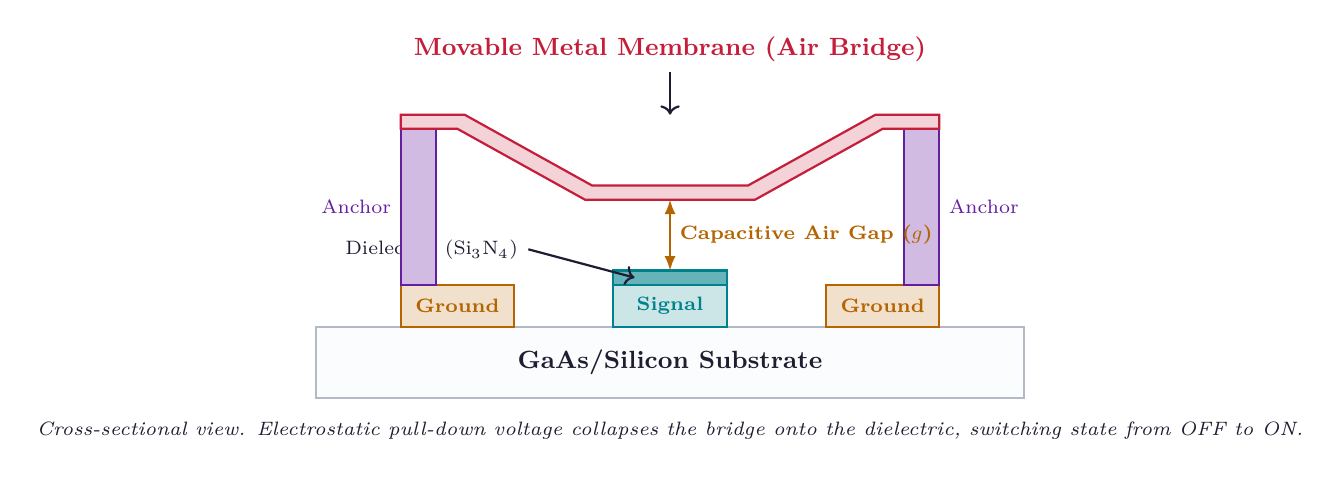
\begin{tikzpicture}[scale=0.9, every node/.style={font=\small}]
  % Substrate
  \draw[thick, fill=mygray!40, draw=mgframe] (0,0) rectangle (10,1.0);
  \node[font=\small\bfseries\color{mydark}] at (5,0.5) {GaAs/Silicon Substrate};

  % CPW Ground Electrodes
  \draw[thick, fill=myamber!20, draw=myamber] (1.2,1.0) rectangle (2.8,1.6);
  \node[font=\scriptsize\bfseries\color{myamber}] at (2.0,1.3) {Ground};
  
  \draw[thick, fill=myamber!20, draw=myamber] (7.2,1.0) rectangle (8.8,1.6);
  \node[font=\scriptsize\bfseries\color{myamber}] at (8.0,1.3) {Ground};

  % CPW Signal Electrode
  \draw[thick, fill=myteal!20, draw=myteal] (4.2,1.0) rectangle (5.8,1.6);
  \node[font=\scriptsize\bfseries\color{myteal}] at (5.0,1.3) {Signal};

  % Dielectric Layer on Signal (CRITICAL for capacitive switch)
  \draw[thick, fill=myteal!60, draw=myteal] (4.2,1.6) rectangle (5.8,1.8);
  \draw[arrow, <-] (4.5, 1.7) -- (3.0, 2.1) node[left, font=\scriptsize] {Dielectric ($\text{Si}_3\text{N}_4$)};

  % Anchors (Left & Right)
  \draw[thick, fill=mypurple!30, draw=mypurple] (1.2,1.6) rectangle (1.7,3.8);
  \draw[thick, fill=mypurple!30, draw=mypurple] (8.3,1.6) rectangle (8.8,3.8);
  \node[left, font=\scriptsize\color{mypurple}] at (1.2,2.7) {Anchor};
  \node[right, font=\scriptsize\color{mypurple}] at (8.8,2.7) {Anchor};

  % Suspended Bridge (Air Bridge Membrane)
  \draw[thick, fill=myred!20, draw=myred] 
    (1.2,3.8) -- (2.0,3.8) -- (3.8,2.8) -- (6.2,2.8) -- (8.0,3.8) -- (8.8,3.8) --
    (8.8,4.0) -- (7.9,4.0) -- (6.1,3.0) -- (3.9,3.0) -- (2.1,4.0) -- (1.2,4.0) -- cycle;

  % Labels and arrows
  \draw[arrow, <-] (5.0, 4.0) -- (5.0, 4.6) node[above, color=myred, font=\small\bfseries] {Movable Metal Membrane (Air Bridge)};
  
  % Capacitive Coupling Air Gap
  \draw[latex-latex, thick, color=myamber] (5.0,1.8) -- (5.0,2.8);
  \node[right, font=\scriptsize\bfseries\color{myamber}] at (5.0, 2.3) {Capacitive Air Gap ($g$)};

  % Switch State description
  \node[below, font=\scriptsize\itshape\color{mydark}] at (5,-0.2) 
    {Cross-sectional view. Electrostatic pull-down voltage collapses the bridge onto the dielectric, switching state from OFF to ON.};
\end{tikzpicture}
\end{tcolorbox}

% ===============================================================================
% MANDATORY QUICK REVISION PAGE
% ===============================================================================
\newpage
\begin{center}
  {\large\bfseries\color{myred} Quick Revision --- Module IX}\\[3pt]
  {\small\color{mydark} Microwave Systems \& Modern Trends $|$ PE-EC701A}
\end{center}
\noindent{\color{myred}\rule{\linewidth}{1.2pt}}
\vspace{4pt}

\begin{tcolorbox}[formulabox, title={\textbf{Key Formulas at a Glance}}]
\renewcommand{\arraystretch}{1.3}
\begin{tabularx}{\linewidth}{B{4.5cm} X}Radar Range Equation   & $R_{\text{max}} = \left[ \frac{P_t G^2 \lambda^2 \sigma}{(4\pi)^3 P_{\text{min}}} \right]^{1/4}$ \\[4pt]
Doppler Frequency Shift & $f_d = \frac{2 v}{\lambda} \cos \theta$ \\[4pt]
Free Space Path Loss    & $\text{FSPL} = \left(\frac{4\pi d}{\lambda}\right)^{\!2}$ \\[4pt]
Specific Absorption Rate& $\text{SAR} = \frac{\sigma |E|^2}{\rho}$ \\[4pt]
Shielding Effectiveness & $\text{SE}_{\text{dB}} \approx A_{\text{dB}} + R_{\text{dB}} + M_{\text{dB}}$
\end{tabularx}
\tcbset{colbacktitle=mygreen, coltitle=white}
\end{tcolorbox}

\begin{tcolorbox}[defbox, title={\textbf{One-Line Definitions}}]
\begin{itemize}[leftmargin=*, itemsep=2.5pt, topsep=0pt]
  \item \textbf{Duplexer:} A fast waveguide switch permitting a single antenna to be shared by radar transmitter and receiver.
  \item \textbf{Doppler Effect:} The change in frequency of a received wave due to relative motion between source and observer.
  \item \textbf{SAR:} Specific Absorption Rate, measuring the rate of electromagnetic energy absorption per unit mass of human tissue.
  \item \textbf{MMIC:} Monolithic Microwave Integrated Circuit, fabricated entirely on a single semiconductor wafer.
  \item \textbf{RFMEMS:} Micro-Electro-Mechanical Systems utilized for high-performance microwave switching and tuning.
  \item \textbf{Triangulation:} Geometric position mapping utilizing measured transit distances from multiple satellites.
  \item \textbf{Clutter:} Unwanted reflections from ground objects, weather, or buildings that interfere with target radar signals.
  \item \textbf{Microwave Imaging:} A non-invasive imaging method mapping dielectric property contrasts within a target.
\end{itemize}
\end{tcolorbox}

\begin{tcolorbox}[exambox, title={\textbf{Frequently Asked / Viva Questions}}]
\begin{enumerate}[topsep=0pt, label=\textbf{Q\arabic*.}, itemsep=5pt]
  \item \Q{Why is a duplexer critical in pulsed radar systems?}
    It isolates the sensitive receiver from the high-power transmitter during the pulse transmission, and routes the weak return echo to the receiver during the rest interval.
  \item \Q{How does Doppler shift change with target movement direction?}
    If the target moves toward the radar, the received frequency increases ($+f_d$). If it moves away, the received frequency decreases ($-f_d$).
  \item \Q{Explain the term "Specific Absorption Rate" (SAR).}
    It is the power absorbed per unit mass of human tissue under RF exposure, measured in W/kg, used to define safety standards for mobile devices.
  \item \Q{What are the advantages of MMICs over hybrid Microwave Integrated Circuits (HMICs)?}
    Small size, low weight, high reliability, ease of mass production, and elimination of wire bond parasitics.
  \item \Q{Describe the function of localizer and glide path transmitters in ILS.}
    The localizer provides horizontal guidance relative to the runway centerline. The glide path provides vertical descent guidance to the runway touchdown point.
  \item \Q{Why does Free Space Path Loss (FSPL) increase with frequency?}
    Because effective antenna aperture decreases as frequency increases ($A_e \propto 1/f^2$), reducing the power intercepted by a matched receiving antenna.
  \item \Q{What are blind speeds in MTI radar and how are they avoided?}
    Blind speeds are target velocities where the Doppler shift matches the radar pulse repetition frequency, making targets appear static. They are avoided by using staggered PRFs.
  \item \Q{What materials are primarily used to fabricate MMICs and why?}
    Gallium Arsenide (GaAs) and Gallium Nitride (GaN) due to high electron mobility, which is necessary for gigahertz operation.
  \item \Q{How does a capacitive RFMEMS switch operate?}
    An electrostatic voltage pulls a suspended metal bridge down onto a dielectric-covered CPW line, dramatically increasing coupling capacitance to short the RF signal.
  \item \Q{Explain how GPS resolves a 3D position using four satellites.}
    Three satellites locate the receiver at the intersection of three spheres. The fourth satellite resolves the clock synchronization error between the receiver and GPS time.
  \item \Q{State the thermal effects of microwaves on the human body.}
    Dielectric heating of water molecules in body tissues, which can lead to localized temperature increases and tissue damage (especially in the eyes and testes).
  \item \Q{What is shielding effectiveness (SE) and what are its main mechanisms?}
    It measures a barrier's ability to attenuate electromagnetic fields, governed by absorption loss, reflection loss, and multiple-reflection corrections.
  \item \Q{Differentiate between active and passive microwave imaging.}
    Active microwave imaging transmits low-power microwave pulses and measures backscattered signals to reconstruct a dielectric profile. Passive microwave imaging uses highly sensitive radiometers to detect the natural thermal electromagnetic radiation emitted by the body.
  \item \Q{Why is microwave imaging promising for breast cancer detection?}
    Because malignant tumors have a high water content and thus show a significant dielectric contrast (permittivity and conductivity are about 5 times higher) compared to normal healthy breast fat tissue. This allows clear imaging without ionizing X-ray radiation.
\end{enumerate}
\tcbset{colbacktitle=mgframe, coltitle=mydark}
\end{tcolorbox}

\begin{tcolorbox}[tikzbox, title={Comparison of MMICs and Hybrid MICs}]
\renewcommand{\arraystretch}{1.4}
\par\noindent
{\renewcommand{\arraystretch}{1.55}%
\begin{tabularx}{\linewidth}{|B{3.2cm}|Y|Y|}\hline
\textbf{Parameter} & \textbf{Monolithic Microwave ICs (MMICs)} & \textbf{Hybrid Microwave ICs (HMICs)} \\[4pt]
\hline
\textbf{Substrate} & Single semiconductor wafer (GaAs, GaN). & Alumina, quartz, or Teflon board. \\
\hline
\textbf{Component Integration} & Transistors and matching lines are grown in-situ on the wafer. & Discrete chips are soldered or wire-bonded to substrate tracks. \\[4pt]
\hline
\textbf{Reliability} & Extremely high (no wire bonds to fail). & Moderate (wire bonds are vulnerable). \\[4pt]
\hline
\textbf{Cost (Low Volume)} & Very High (complex mask tooling). & Moderate (easy prototyping). \\
\hline
\textbf{Cost (High Volume)} & Very Low (mass batch production). & High (requires manual/auto assembly). \\[4pt]
\hline
\end{tabularx}
}
\end{tcolorbox}


\end{document}
